%\documentclass[12pt,twoside]{book}
\documentclass[12pt,twoside]{report}
\usepackage[utf8]{inputenc}
\usepackage[english]{babel}
\usepackage[x11names,dvipsnames,table,xcdraw,svgnames]{xcolor}
\usepackage[margin=1in]{geometry}
\usepackage[T1]{fontenc}
\usepackage{mathtools}
\usepackage{amsmath,amsfonts,amssymb,bm}
\usepackage{subcaption}
\usepackage{graphicx}
\usepackage{float}
\usepackage[colorinlistoftodos]{todonotes}
%\usepackage{subfig}
\usepackage[labelfont=bf]{caption}
\usepackage[nohints]{minitoc}
\usepackage[toc,page]{appendix}
\usepackage{afterpage}
\usepackage{eso-pic}
\usepackage{fancyhdr}
\pagestyle{fancy}
\fancyhf{}
\usepackage{lastpage}
\setlength{\parindent}{0pt}
\usepackage{esvect}
\usepackage{nicefrac}
\usepackage{listings}
\usepackage{tocloft}
\usepackage{enumitem}
\usepackage{calc}
\usepackage{marvosym}
\usepackage{multirow}
\usepackage[colorlinks,linktocpage]{hyperref}
\usepackage[most]{tcolorbox}
\usepackage{boxhandler}
\usepackage{gensymb}
\usepackage{lipsum}
\usepackage{booktabs}
%\usepackage{chemist}
\usepackage{textcomp}
\usepackage{pdfpages}
\usepackage{emptypage}
\usepackage{array}
\usepackage{tikz}
\usepackage{tikz-layers}
\usepackage{pgfplots}
\pgfplotsset{compat = newest}
\usetikzlibrary{patterns,decorations.pathmorphing,positioning}
\usetikzlibrary{shapes.geometric}
\usetikzlibrary{calc,angles,quotes}
\usetikzlibrary{trees}
\usetikzlibrary{mindmap}
\usetikzlibrary{pgfplots.groupplots}
\usetikzlibrary{arrows.meta}
\usetikzlibrary{intersections, pgfplots.fillbetween}
\usetikzlibrary{plotmarks}
\usepackage[compact]{titlesec}
\usepackage{adforn} % \adforn{21}\quad\adforn{11}\quad\adforn{49}
\usepackage{pgfornament}
%\usepackage[super]{nth}
%\usepackage[capitalise,noabbrev,nameinlink]{cleveref}
\usepackage[round]{natbib}
%\bibliographystyle{unsrtnat}
\bibliographystyle{plainnat}
\usepackage[percent]{overpic}
\usepackage[edges]{forest}
\usepackage{sectsty}
\usepackage{floatrow}
\usepackage[ruled,vlined,english, algosection]{algorithm2e}
\usepackage{svg}
\usepackage{makecell}
\setsvg{inkscape=inkscape -z -D, svgpath=images/}
% eps2pdf



%%%%%%%%%%%%%%%%%%%%%%%%%%%%%%%%%%%%%%%%%%%%
%   Reduce the margin of the summary:
\def\changemargin#1#2{\list{}{\rightmargin#2\leftmargin#1}\item[]}
\let\endchangemargin=\endlist 

%   Generate the environment for the EN_abstract:
\newcommand\summaryname{Abstract}
\newenvironment{abstract}%
    {\small
    \begin{center}%
    \bfseries{\summaryname} \end{center}}
    
%   Generate the environment for the FR_abstract:
\newcommand\summarynameFR{Résumé}
\newenvironment{abstract_fr}%
    {\small
    \begin{center}%
    \bfseries{\summarynameFR} \end{center}}
%%%%%%%%%%%%%%%%%%%%%%%%%%%%%%%%%%%%%%%%%%%%%

\newcommand\blankpage{%
    \null
    \thispagestyle{empty}%
    \addtocounter{page}{-1}%
    \newpage}
    
%%%%%%%%%%%%%%%%%%%%%%%%%%%%%%%%%%%%%%%%%%%%%%

\hypersetup{
    colorlinks=true,
    citecolor=Green,
    filecolor=black,
    linkcolor=blue,
    urlcolor=MidnightBlue,
    pdftitle={Mémoire de stage - 3ème année cycle ingénieur - Tom MOUSSIE}
}

%%%%% NO HYPHEN IN TEXT %%%%%%%
\tolerance=1
\emergencystretch=\maxdimen
\hyphenpenalty=10000
\hbadness=10000
%%%%%%%%%%%%%%%%%%%%%%%%%%%%%%%


\renewcommand \pd[2] { \frac{\partial {#1} } {\partial {#2}} }
\newcommand{\Reynolds}{$Re$ }
\newcommand{\keps}{$\mathcal{K}-\varepsilon$ }
\newcommand{\kom}{$\mathcal{K}-\omega$ }
\newcommand{\Hx}{\mathcal{H}\mathbf{x} }


%%%%%%%%%%%%%%%%%%%%%%%%%%%%%%%%%%%%%%%%%%%%
\newcommand{\Autoref}[1]{%
  \begingroup%
    \def\chapterautorefname{Chapter}%
    \def\sectionautorefname{Section}%
    \def\subsectionautorefname{Subsection}%
    \def\subsubsectionautorefname{Subsubsection}%
    \def\paragraphautorefname{Paragraph}%
    \def\tableautorefname{Table}%
    \def\equationautorefname{Equation}%
    \def\algorithmautorefname{Algorithm}%
    \def\lineautorefname{Step}%
  \autoref{#1}%
  \endgroup%
}

\newcommand{\Autorefs}[1]{%
  \begingroup%
    \def\chapterautorefname{Chapters}%
    \def\figureautorefname{Figures}%
    \def\sectionautorefname{Sections}%
    \def\subsectionautorefname{Subsections}%
    \def\subsubsectionautorefname{Subsubsections}%
    \def\paragraphautorefname{Paragraphs}%
    \def\tableautorefname{Tables}%
    \def\equationautorefname{Equations}%
    \def\algorithmautorefname{Algorithms}%
    \def\lineautorefname{Lines}%
  \autoref{#1}%
  \endgroup%
}
%%%%%%%%%%%%%%%%%%%%%%%%%%%%%%%%%%%%%%%%%%%%%

\usepackage[acronym, automake]{glossaries-extra}
\setabbreviationstyle[acronym]{long-short}
\renewcommand*{\glstextformat}[1]{\textcolor{darkgray}{#1}}
\makeglossaries

%%%%%%%%%%%%%%%%%%%%%%%%%%%%%%%%%%%%%%%%%%%
%%%%%%%%%%%% ABRÉVIATIONS %%%%%%%%%%%%%%%%%
%%%%%%%%%%%%%%%%%%%%%%%%%%%%%%%%%%%%%%%%%%%

\newacronym{cfd}{CFD}{Computational Fluid Dynamics}
\newacronym{barc}{BARC}{Benchmark on the Aerodynamics of a Rectangular Cylinder}
\newacronym{les}{LES}{Large Eddy Simulation}
\newacronym{rans}{RANS}{Reynolds Average Navier Stokes}
\newacronym{des}{DES}{Detached-Eddy Simulation}
\newacronym{ddes}{DDES}{Delayed Detached Eddy Simulation}
\newacronym{iddes}{IDDES}{Improved Delayed Detached Eddy Simulation}
\newacronym{hpc}{HPC}{High Performance Computing}
\newacronym{ensam}{ENSAM}{École Nationale Supérieure des Arts et Métiers}
\newacronym{lml}{LML}{Laboratoire de Mécanique de Lille}
\newacronym{lamcube}{LaMcube}{Laboratoire de Mécanique, Multiphysique, Multiéchelle}
\newacronym{lmfl}{LMFL}{Laboratoire de Mécanique des Fluides de Lille - \textit{Kampé de Fériet}}
\newacronym{uml}{UML}{Unité de Mécanique de Lille - \textit{J. Boussinesq}}
\newacronym{dns}{DNS}{Direct Numerical Simulations}
\newacronym{sgs}{SGS}{sub-grid scale}
\newacronym{cstb}{CSTB}{Centre Scientifique et Technique du Bâtiment}
\newacronym{tke}{TKE}{Turbulence Kinetic Energy}
\newacronym{da}{DA}{Data Assimilation}
\newacronym{kf}{KF}{Kalman Filter}
\newacronym{enkf}{EnKF}{Ensemble Kalman Filter}
\newacronym{cwt}{CWT}{Continuous Wavelet Transform}
\newacronym{nrmsd}{NRMSD}{Normalized Root-Mean-Square Deviation}
\newacronym{cad}{CAD}{Computer-Aided Design}
\newacronym{menkf}{MEnKF}{Multigrid Ensemble Kalman Filter}
\newacronym{cnrs}{CNRS}{Centre National de la Recherche Scientifique}
\newacronym{onera}{ONERA}{Office National d'Études et de Recherches Aérospatiales}
\newacronym{ram}{RAM}{Random Access Memory}


%%%%%%%%%%%%%%%%%%%%%%%%%%%%%%%%%%%%%%%%%%%
%%%%%%%%%%%%%% GLOSSAIRE %%%%%%%%%%%%%%%%%%
%%%%%%%%%%%%%%%%%%%%%%%%%%%%%%%%%%%%%%%%%%%

\newglossaryentry{maths}
{
        name=mathematics,
        description={Mathematics is what mathematicians do}
}



%%%%%%% OTHER MINOR FORMATTING %%%%%%%%%%%%%%
\titleformat{\chapter}[display]
{\normalfont\Huge\bfseries}{\chaptertitlename\ \thechapter}{20pt}{\Huge}

\DeclareUnicodeCharacter{20AC}{\EUR{}}

\counterwithout{footnote}{chapter}

\raggedbottom % Evite que le texte soit justifié verticalement avec la class "book"

\newcolumntype{C}[1]{>{\centering\let\newline\\\arraybackslash\hspace{0pt}}m{#1}}


%%%%%%%%%%%%%% FOREST TREE FORMAT %%%%%%%%%%%%%%%

\definecolor{folderborder}{RGB}{110,144,169}
\definecolor{folderbg}{rgb}{0.91, 0.84, 0.42}
\newlength\Size
\setlength\Size{4pt}
\tikzset{%
  folder/.pic={%
    \filldraw [draw=folderborder, top color=folderbg!50, bottom color=folderbg] (-1.05*\Size,0.2\Size+5pt) rectangle ++(.75*\Size,-0.2\Size-5pt);
    \filldraw [draw=folderborder, top color=folderbg!50, bottom color=folderbg] (-1.15*\Size,-\Size) rectangle (1.15*\Size,\Size);
  },
  file/.pic={%
    \filldraw [draw=folderborder, top color=folderborder!5, bottom color=folderborder!10] (-\Size,.4*\Size+5pt) coordinate (a) |- (\Size,-1.2*\Size) coordinate (b) -- ++(0,1.6*\Size) coordinate (c) -- ++(-5pt,5pt) coordinate (d) -- cycle (d) |- (c) ;
  },
}
\forestset{%
  declare autowrapped toks={pic me}{},
  pic dir tree/.style={%
    for tree={%
      folder,
      font=\footnotesize \ttfamily,
      grow'=0,
    },
    before typesetting nodes={%
      for tree={%
        edge label+/.option={pic me},
      },
    },
  },
  pic me set/.code n args=2{%
    \forestset{%
      #1/.style={%
        inner xsep=2\Size,
        pic me={pic {#2}},
      }
    }
  },
  pic me set={directory}{folder},
  pic me set={file}{file},
}
\newcommand\fname[2]{#1}

\forestset{
  arrow to next tree/.code={
    \draw[dashed] (current bounding box.south east) -- ++(1.5em,0);
    \draw[->](current bounding box.south east) ++(0.25em,0) -- ++(1.5em,0) -- (current bounding box.north east) -- ++(1.5em,0);
  },
  dots below/.style={
    for group={#1}{
      tempdima/.option=y,
      for next node={
        for ancestors={
          TeX={%
            \draw([xshift=\forestregister{folder indent}].parent anchor)--([xshift=\forestregister{folder indent}]\forestoption{x},\forestregister{tempdima}) node[anchor=north]{\vdots};
          },
        },
      },
    },
  },
  prepare fake ancestors/.style={
    for group={#1}{
      init prepare fake parent,
      prepare fake ancestors',
    },
  },
  prepare fake ancestors'/.style={
    if nodewalk valid={parent}{
      for parent={
        prepare fake parent,
        prepare fake ancestors',
      },
    }{},
  },
  init prepare fake parent/.style={
    tempdima/.option=y,
  },
  prepare fake parent/.style={
    y/.register=tempdima, y+=10pt,
    coordinate, edge label={}, no edge,
    tikz={\node at ()[anchor=south,xshift=\forestregister{folder indent}]{\vdots};},
    typeset node,
  },
  draw part of tree/.style 2 args={
    for nodewalk={#1,tempcounta/.option=id}{},
    for nodewalk={#2,tempcountb/.option=id}{},
    draw@part@of@tree/.process=RR{tempcounta}{tempcountb},
  },
  draw@part@of@tree/.style 2 args={
    draw tree processing order/.nodewalk style={
      id=#1,
      ancestors,
      fake={id=#1},
      do until={id()==#2}{next node},
    },
    for root'={
      post draw tree hook/.style={},
      for id={#2}{
        if nodewalk valid={next node}{
          post draw tree hook/.append style={
            to be continued={id=#1}{id=#2},
          },
        }{}
      },
      prepare fake ancestors={id=#1},
      draw tree,
    },
  },
  declare count register=current first node,
  draw linear split tree/.style={
    draw tree method/.append style={post draw tree hook},
    begin draw/.append code={[baseline=(current bounding box.north)]},
    draw tree stage/.style={},
    for root'={current first node/.option=id},
    before typesetting nodes/.process=Ow{id}{
      draw tree stage/.append style={
        draw part of tree={id/.register=current first node}{root',last leaf},
      },
    },
  },
  split here/.style={
    draw tree stage/.append style/.process=ROw2{current first node}{id}{
      draw part of tree={id=##1}{id=##2,previous node},
    },
    current first node/.option=id,
  },
}


\makeatletter
\@addtoreset{section}{part}
\makeatother
\newlength\mylen
\renewcommand\thepart{\arabic{part}}
\renewcommand\cftpartpresnum{Part~}
\settowidth\mylen{\bfseries\cftpartpresnum\cftpartaftersnum}
\addtolength\cftpartnumwidth{\mylen}
\renewcommand{\thepart}{\Roman{part}} 
%%%%%%%%%%%%%%%%% BEGIN DOCUMENT %%%%%%%%%%%%%%%

\begin{document}
%\selectlanguage{french}
%\mtcselectlanguage{french}
\dominitoc

%EN-TETE
\renewcommand\headrulewidth{0.5pt}
\fancyhead[LE,RO]{\textsl{\scriptsize{\leftmark}}}

%PIED DE PAGE
\renewcommand\footrulewidth{0.5pt}
\fancyfoot[RE,LO]{{Page \thepage}}
%\cfoot{\thepage} %\ / \pageref{LastPage}}
%\fancyfoot[RE,LO]{\textcolor{red}{Confidentiel}}

%FANCY HDR POUR LES PAGES DE CHAPTER
\fancypagestyle{plain}{%  first page of chapters
    \fancyhf{} % clear all header and footer fields
    \fancyfoot[RE, LO]{Page \thepage}
    %\fancyfoot[RE, LO]{{\textcolor{red}{Confidentiel}}}
    \renewcommand{\headrulewidth}{0pt} % no header rule
    \renewcommand{\footrulewidth}{0pt} % no footer rule
}

% FANCY HDR FOR REMERCIEMENTS, AVERTISSEMENTS, ...
\fancypagestyle{before_TOC_style}
{
    \fancyhf{} % clear all header and footer fields
    \fancyfoot[RE, LO]{{\textcolor{red}{Confidentiel}}}
    \renewcommand{\headrulewidth}{0pt} % no header rule
    \renewcommand{\footrulewidth}{0pt} % no footer rule
}

\begin{titlepage}

\newcommand{\HRule}{\rule{\linewidth}{0.25mm}}
\newcommand{\HRuleA}{\rule{\linewidth}{0.5mm}}
\newcommand{\HRuleB}{\rule{\linewidth}{1mm}}

\center 
 
%-------------------------------------%
%	       REPORT SUBJECT
%-------------------------------------%

\begin{table}[h!]
\makebox[\textwidth][c]{
\centering
\begin{tabular}{C{5.2cm} C{5.2cm} C{5.2cm}}
\footnotesize
\begin{tabular}[c]{@{}c@{}}\textsc{Institut Polytechnique}\\ \textsc{des Sciences Avancées} \\[0.5cm] 63 Bd de Brandebourg Bis \\ 94200 Ivry-sur-Seine\end{tabular} & %
\footnotesize
\begin{tabular}[c]{@{}c@{}}\textsc{Laboratoire de Mécanique}\\ \textsc{des Fluides de Lille} \\[0.5cm] 8 Bd Louis XIV \\ 59000 Lille\end{tabular} & %
\footnotesize
\begin{tabular}[c]{@{}c@{}}\textsc{École Nationale Supérieure}\\ \textsc{des Arts et Métiers}\\[0.5cm] 8 Bd Louis XIV \\ 59000 Lille\end{tabular} 
\end{tabular}}
\label{tab:my-table}
\end{table} 

\vspace*{3cm}

\AddToShipoutPicture*
{\put(115,600){\includegraphics[width=2.5cm]{images/ipsa-logo.png}}}

\AddToShipoutPicture*
{\put(395,575){
\includegraphics[width=5cm]{images/Logo_couleur_RVB.png}}}

\AddToShipoutPicture*
{\put(257.5,600){\includegraphics[width=3.5cm]{images/lmfl.png}}}

%\AddToShipoutPicture*
%{\put(342.5,623.5){\includegraphics[width=5cm]{images/logoADHEX.png}}}

%-------------------------------------------
%	TITLE SECTION
%--------------------------------------------

\HRule\\[0.33cm]

\textbf{{\LARGE Data-driven inference of unsteady inlet \\ conditions for the numerical simulation \\[0.4cm] of the BARC test case}} \\[0.25cm]
% \pgfornament[width = 2cm, color = black]{75} \\[0.25cm]
\textsc{\normal End-of-study thesis for engineering degree}\\[0.25cm]
 \begin{figure}[h!]
     \centering
     \includegraphics[width=.65\textwidth]{images/face_pic.png}
 \end{figure}
\HRule

%----------------------------------------
%	AUTHOR SECTION
%-----------------------------------------
\begin{center}
    \textsc{\textbf{Tom MOUSSIE}} \\
    \textsl{Aerospace Vehicles} Major \\
    \textsl{Aeronautic Cells} Specialization\\[0.75cm]
    Educational tutor : \textbf{Pierre-Élie WEISS}\\
    Laboratory tutor : \textbf{Marcello MELDI}\\[0.75cm]
    Internship period : \textbf{February 6$^{\text{th}}$ 2023} - \textbf{July 21$^{\text{st}}$ 2023} \\
    Academic Year : \textbf{2022 - 2023}\\[0.75cm]
    \textcolor{red}{\textbf{Final version of \today}}
    %\Huge{\textcolor{red}{\textbf{\textsc{Confidentiel}}}}
\end{center}

%-------------------------------------
%	DATE SECTION
%-------------------------------------

\vfill
\end{titlepage}

%\afterpage{\blankpage} 
%Création d'une page vide pour le style du document

\chapter*{Foreword}
\thispagestyle{empty}
The writing of this thesis is complete. \\
It is therefore the final version as of \today.




\clearpage

\chapter*{Acknoledgments}
%\thispagestyle{before_TOC_style}
\thispagestyle{empty}

First and foremost, let me thank the Laboratoire de Mécanique des Fluides de Lille for allowing me to carry out my end-of-study internship among their research teams. Thanks should also go to École Nationale Supérieure des Arts et Métiers for hosting me during the last six months. \\

To begin with, I would like to express my deepest gratefulness to my laboratory tutor, Marcello MELDI. His mentorship and expertise have been some precious assets all during the internship. Marcello's  knowledge and experiences in research allowed me to spend a fascinating internship full of perspectives in the academic domain. His dedication to his students, both trainees and PhD, gave me a feeling of solid guidance while allowing me freedom of thought and reflection. \\

I am extremely grateful to Miguel MARTÍNEZ VALERO who allowed me to perfectly being integrated into the laboratory from the very start of my internship, and without whom this journey would not have been the same. Miguel always had the time to answer my questions, and his great knowledge allowed me to work in the best possible conditions. \\

I would like to extend my sincere thanks to Paolo ERRANTE for his technical support throughout the internship period. Paolo introduced me to numerous technical tools that will be with me for the years to come and ensured that I could work in the best possible conditions and without any technical problems. Our many discussions gave me new food for thought and solved many of the problems I was facing. \\

I would also like to acknowledge Antoine DAZIN, Pierric JOSEPH and Francesco ROMANÒ for their warm welcome. They made me feel at ease from the moment I arrived. I had the pleasure of collaborating with all the PhD students, with whom I spent nice moments whether for scientific talking or outside work. \\

Many thanks to Pierre-Élie WEISS, my educational tutor and teacher at IPSA, who really took the time to follow the different stages of my internship. \\

Lastly, I would be remiss in not mentioning my parents, who have been supporting me during these last 5 years. They provided me with their full dedication and commitment, for which I am extremely grateful.


%\addcontentsline{toc}{chapter}{Remerciements}
%\addstarredchapter{Remerciements}

\clearpage
%\afterpage{\blankpage} 

% \chapter*{Caution}
% \thispagestyle{before_TOC_style}



\clearpage

\tableofcontents
% {\pagestyle{plain} \tableofcontents \doubleclearpage \thispagestyle{empty}}
\addtocontents{toc}{\protect\thispagestyle{empty}}
\thispagestyle{empty}


\pagenumbering{roman}
%\chapter*{Fiche de synthèse}
\thispagestyle{empty}
\begin{center}
	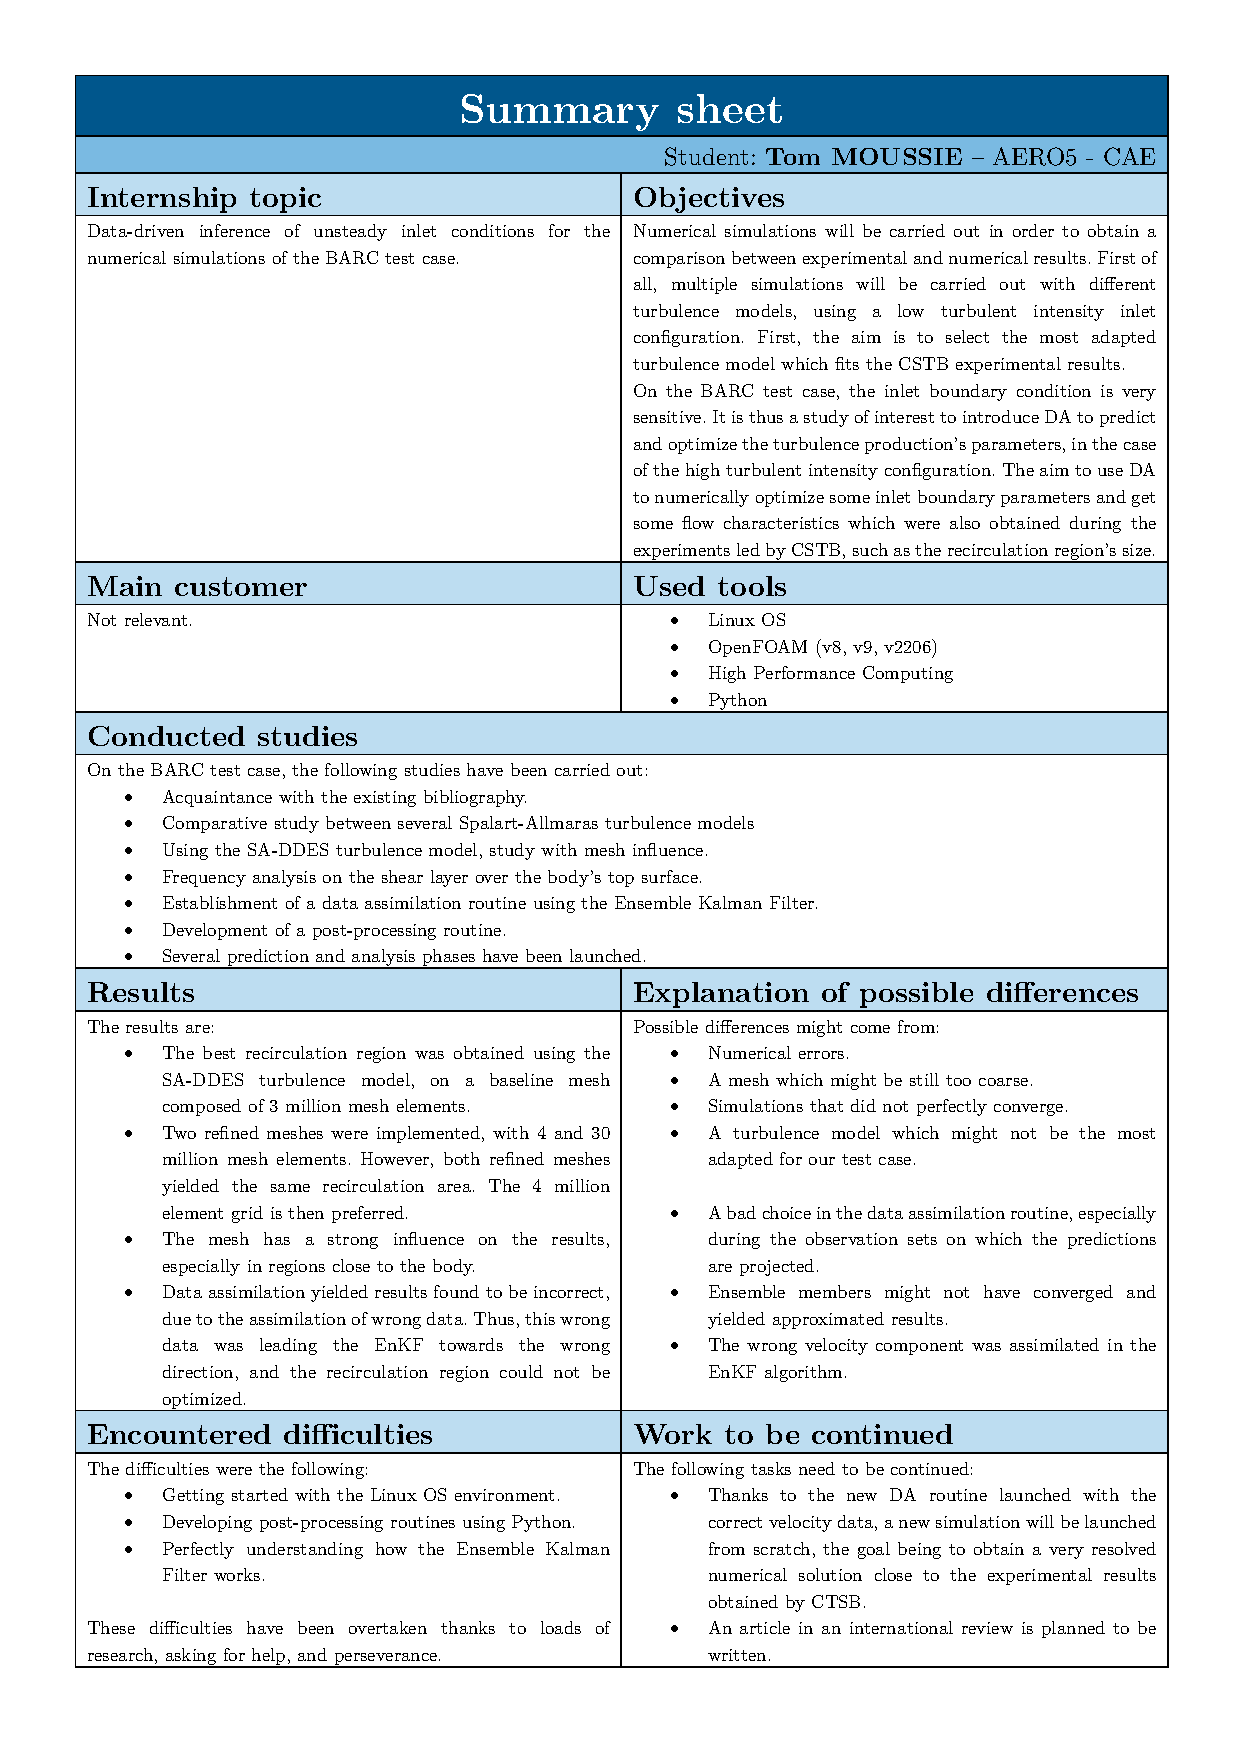
\includepdf[pages=-,scale=.99]{summary_sheet.pdf}
\end{center}





%\addstarredchapter{Fiche de synthèse}

\clearpage
\pagenumbering{arabic}
\setcounter{page}{1}

\part{Establishment}

\clearpage

\chapter{Introduction}

\minitoc

\clearpage 

\section{Case study presentation}
The \gls{barc} is a well-known test case in fluid mechanics literature, used to examine the key characteristics of external flows found in transportation engineering and urban settings. During the latest decades, access to numerical resources has considerably increased, which enables the fluid mechanics research field to perform a growing amount of numerical simulations for automotive and aeronautics, but also for urban environments. The \gls{barc} is thus a popular study case of a simplified urban flow, with which the analogy can be made with many urban structures. 

Despite its simple appearance, this configuration, as illustrated in \autoref{fig:BARC_geometry}, involves complex physical processes such as boundary layer separation, flow reattachment, recirculation zones, and Von Karman streets, which impact the propagation of acoustic waves and the flow's structural organization. To accurately predict the behaviour of practical systems, it is crucial to fully comprehend these mechanisms and their interactions. One major challenge in studying this flow through numerical methods is its sensitivity to the geometric characteristics and boundary conditions, particularly the velocity field imposed at the inlet. This is especially true for scale-resolving approaches like \gls{les}, which is now widely used for analyzing bluff bodies.
\begin{figure}[h!] 
    \centering
    \includegraphics[width=.95\textwidth]{images/BARC_lmfl.png}
    \caption{\gls{barc} geometry sketch, with the reference system and the computational domain employed in the present work.}
    \label{fig:BARC_geometry}
\end{figure}

This study is carried out in a context of validation of experimental data recently performed by the \gls{cstb}\footnote{\url{https://recherche.cstb.fr/fr/}}. Through their wind tunnel, the research teams have developed a \gls{barc} test case experiment with two different configurations which respectively have a low and a high turbulent intensity. 

Thus, numerical simulations will be carried out in order to obtain a comparison between experimental and numerical results. First of all, multiple simulations will be carried out with different turbulence models, using the low turbulent intensity configuration. The aim is to select the most adapted turbulence model which fits the \gls{cstb} experimental studies. \\

On the \gls{barc} test case, the inlet boundary is very sensitive. It is thus a study of interest to introduce \gls{da} to predict and optimize the turbulence production's parameters, in the case of the high turbulence intensity configuration. The aim is to use \gls{da} to numerically optimize some inlet boundary parameters and get some flow characteristics which were also obtained during the experiments led by \gls{cstb}. \gls{da} is a powerful set of tools and methods used to reach an accurate estimation of a system by coupling experimental observations and numerical simulations. These methods have already proved their worth in numerous scientific fields, but their usage in \gls{cfd} is recent, which makes \gls{da} an expanding topic in fluid mechanics research. 

\section{Internship presentation}
This end-of-study internship puts an end to my studies at IPSA. For the last 5 years, I have been specializing in aeronautical engineering, and this internship aims to apply my theoretical and technical skills. My various academic and professional experiences led me to discover the field of research, and more particularly research in fluid dynamics. Indeed, I particularly appreciated discovering \gls{cfd} during my studies and this is the reason why I wanted to realize this internship in this field. 

\begin{figure}[h!]
    \centering
    \includegraphics[width=0.5\textwidth]{images/Ensam_vue_ciel.jpg}
    \caption{Arts et Métiers Lille, view from the sky.}
    \label{fig:ENSAM_sky}
\end{figure}

% Dates du stage, endroit du stage, poste occupé
During the last six months, I have been hosted by \gls{ensam}, more precisely at Lille campus. Arts et Métiers is known to be a prestigious engineering school with a focus on mechanics, industrial and energy engineering. Its Lille campus offers students unique opportunities to study in a dynamic and innovative environment, located in the heart of a region known for its industrial history. \\

% Décrire brièvement le sujet du stage


\section{Laboratory presentation}
% Histoire scientifique de la région Lilloise
Historically, Lille had a very strong link with scientific culture for over 100 years. Prominent scientific names have taught at Lille University, such as Joseph Boussinesq in the 1870 decade, and Joseph Kampé de Fériet between 1919 and 1969. Engineering and research education has known a major expansion at the end of the XIX$^{\text{th}}$ and the beginning of the XX$^{\text{th}}$ century, thanks to the \textsl{Institut Industriel du Nord} extension and \textsl{Arts et Métiers} creation. \\

% Histoire du laboratoire
Created in 1985, the \gls{lml} was gathering research teams from different domains such as mechanics or civil engineering from \textsl{Arts et Métiers}, \textsl{Ecole Centrale de Lille} and \textsl{Lille University}. The \gls{lml} disappeared in 2017 and the 200 researchers and students were split into three new laboratories:
\begin{itemize}
    \item[$-$] \gls{lamcube}
    \item[$-$] \gls{lmfl}
    \item[$-$] \gls{uml}
\end{itemize}

% Effectif du laboratoire 
Geographically present on the sites of \gls{ensam}, \gls{onera} and \gls{cnrs}, the  \gls{lmfl} research unit has 38 permanent staff and nearly 25 PhD and post-doctoral students. 

\begin{figure}[h!]
    \centering
    \includegraphics[width=.7\textwidth]{images/lmfl_collage-1200x547.jpg}
    \caption{\gls{lmfl} facilities. Top:Villeneuve d’Ascq’s campus gathering \textsl{Centrale Lille}, \gls{cnrs} and \textsl{Univsersité de Lille}. Bottom-left: \gls{onera}. Bottom-right: \gls{ensam}.}
    \label{fig:LMFL_facilities}
\end{figure}

% Les labos de l'ENSAM Lille:
In addition to providing engineering training, the Lille campus of \gls{ensam} houses four research laboratories in various fields: electrical engineering (L2EP - Laboratoire d’électrotechnique et électronique de puissance), collaborative robotics (LISPEN - Laboratoire d’ingénierie des systèmes physiques et numériques), vibratory mechanics, materials and processes (MSMP - Laboratoire Mechanics, Surfaces and Materials Processing) and fluid mechanics (\gls{lmfl}). 

\clearpage

This diversity of skills allows the research teams to be involved in numerous partnership projects in connection with regional or national structures.
\begin{figure}[t!]
	\centering
	\includegraphics[width=.6\textwidth]{images/IMG_7963.JPEG}
	\caption{\gls{lmfl} facility inside \gls{ensam} enclosure.}
	\label{fig:lmfl_inside_ensam}
\end{figure}

% Activités du LMFL
Research conducted within the \gls{lmfl} is organized into three main topics:
\begin{enumerate}
    \item \textbf{Turbulence: } Studying and modeling turbulent flows using numerical and experimental methods. A focus is made on inhomogeneity and non-stationarity in wall-bounded flows, wakes, jets and several other flow configurations. This research theme gathers 5 permanent researchers and about 10 PhD and post-doctoral students.
    \begin{figure}[h!]
    		\centering
    		\includegraphics[width=.75\textwidth]{images/turbulence_LMFL.png}
    		\caption{Turbulence research conducted at \gls{lmfl}. Pictures from left to right: mixer, wakes, jets.}
    		\label{fig:turbulence_LMFL}
    \end{figure}
    \item \textbf{Rotating flows: } Analyzing and modeling internal and external flows related to rotating machines, such as turbo-machinery and rotors. Experimental and numerical study of rotating machines (turbomachines, rotors, propellers) operating in degraded conditions, flow control, cavitation and multiphase flows are also topics of great interest. This subject gathers 6 researchers, 7 research engineers and about 13 PhD and post-doctoral students.
    
  
\clearpage    


    \begin{figure}[t]
    		\centering
    		\includegraphics[width=.76\textwidth]{images/rotating_LMFL.png}
    		\caption{\textsl{CME2} rotating machinery at \gls{lmfl}. Pictures from left to right: \textsl{CME2} \gls{cad} model, \textsl{CME2} rotor\,/\,stator.}
    		\label{fig:rotating_LMFL}
    \end{figure}

    
    \item \textbf{Flight dynamics in unsteady and non-uniform environments: } Development of analytical and experimental methods to determine the evolving behaviour of low-speed aircrafts in perturbed flight domains. Dynamic of post-stall behaviour, interaction with the environment and definition of experiments are subjects of interest. This topic gathers about 5 research engineers and 5 PhD and post-doctoral students.
        \begin{figure}[h!]
    		\centering
    		\includegraphics[width=.6\textwidth]{images/aerodyn_LMFL.png}
    		\caption{Flight dynamics research at \gls{lmfl}. Pictures from left to right: \gls{cfd} simulation, corresponding experimental montage.}
    		\label{fig:aerodyn_LMFL}
    \end{figure}
\end{enumerate}

Three other cross-cutting topics are studied in the laboratory:
\begin{enumerate}
    \item \textbf{Optical metrology: } Method and algorithm development for optical measurements in turbulent flows. 
    \item \textbf{Active flow control: } Active control method and algorithm development for internal and external flows.
    \item \textbf{Data analysis: } Tool development and characterization for turbulent flow studying, with methodology development for data enrichment. \\
\end{enumerate}

%\gls{lmfl} also includes a factory floor in which can be found machineries.
%\begin{figure}[h!]
%    \begin{subfigure}[t]{.48\textwidth}
%    \centering
%    \includegraphics[width=\linewidth]{images/IMG_7994.JPEG}
%    \caption{}
%    \label{fig:}
%  \end{subfigure}
%  \hfill
%  \begin{subfigure}[t]{.48\textwidth}
%    \centering
%    \includegraphics[width=\linewidth]{images/IMG_7995.JPEG}
%    \caption{}
%    \label{fig:}
%  \end{subfigure}
%    \caption{Machineries available at \gls{lmfl}}
%  \label{fig:}
%\end{figure}

\clearpage

\section{Organigram}

The \gls{lmfl} is structred according to the following organization chart:
\begin{figure}[h!]
	\centering
	\includegraphics[width=\textwidth]{images/orga_LMFL.png}
	\caption{\gls{lmfl} organization chart.}
	\label{fig:LMFL_organigramme}
\end{figure}



\clearpage

%% 1. CFD of hybrid RANS - LES model (DDES, IDDES) --> compare experiments of DDES, IDDES and IDDES no wall modeling simulations

%% 2. DA (Data Assimilation) : CFD + Exp. (Penalization?)

%% 3. DA : IBM CFD + Exp. ==> CICLONE

% \part{CFD simulations using hybrid models}




\clearpage

\chapter{State of the art} \label{ch:state_of_the_art}
%%% Rappel de la problématique %%%

% 
Introduced during the VI Colloquium on Bluff Body Aerodynamics and Applications (BBAA VI, 2008), \gls{barc}'s objective is to create discussions between researchers and scientists about bluff body aerodynamics, and more specifically about turbulence and separated flows. As for the research interest previously depicted, the benchmark's industrial applications cover a wide engineering range, such as civil engineering with long-span bridges and skyscrapers. \\

The \gls{barc} test case has been a subject of great interest over the past decades, even before it has been officially announced. Despite its simple geometry, its configuration allows the observation of three-dimensional complex phenomena, such as turbulence, flow separation and reattachment. Moreover, the interaction between small and large-scale processes makes these studies particularly relevant. \\



%%% Description des différents travaux déjà effectués %%%

\section{\glsxtrfull{barc}}

Experimental studies have highlighted the influence of parameters which have a preponderance on the results. Prior to \gls{barc} announcement, numerous experimental studies have been conducted, in which breadth ($B$) to depth ($D$) ratios $\nicefrac{B}{D}$ from 0.2 to 52, a Reynolds number from 200 to 300\,000 was implemented. The different studies carried out are gathered in \cite{bruno_benchmark_2014}. \\

With $\nicefrac{B}{D}$=5, \cite{ricciardelli_sectional_2008} concluded that the nature of the flow had influenced the distribution of the pressure field on the lateral faces. The pressure fluctuations then indicate the position of the reattachment and thus of the recirculation bubble. In the case of a turbulent regime, the separation is shorter and the reattachment of the flow thus moves away from the trailing edge.

\clearpage

\cite{haan_anatomy_2009} showed turbulence effects on an oscillating rectangular prism, more especially for self-excited and buffeting forces. A ratio of $\nicefrac{B}{D}$ equal to 6.67 has been used. \\

A first deep spectral study was led by \cite{le_spanwise_2009}, focusing on conventional Fourier and wavelet transforms to understand turbulence, with turbulent intensities going from 9.5\,\% to 11.5\,\%. Using ratios of $\nicefrac{B}{D}$=1 and $\nicefrac{B}{D}$=5, and \Reynolds from 18\,000 to 54\,000, investigations on the spanwise separation and Karman vortices, among others, are made. It has been concluded that the side ratio $\nicefrac{B}{D}$ is suggested as one parameter relating to the effect of the bluff body flow in the force coherence for cases of rectangular cylinders. \\

\cite{ricciardelli_effects_2010} used a $\nicefrac{B}{D}$ ratio of 5, with a \Reynolds$=64\,000$. Measurements were carried out on the stationary cylinder and in four dynamic configurations, each characterized by different values of the heaving and pitching natural frequencies. The results show how the amplitude of oscillation is not the only parameter that influences the correlation of the aerodynamic pressures and forces, as this depends also on the degree of freedom in which the cylinder oscillates. \\

\vspace*{0.5cm}

As well as experimental studies, numerical studies have been conducted prior to the \gls{barc}’s announcement. One can mention in particular \cite{yu_parametric_1998} in which a \gls{les} simulation is conducted using a \Reynolds $=10^5$ and different aspect ratios $\nicefrac{B}{D}$ from 1 to 4. The Smagorinsky turbulence model has been used for representing the \gls{sgs} viscosity.  \\

A \gls{rans} simulation was led by \cite{shimada_application_2002}, in which various $\nicefrac{B}{D}$ ratios ranging from 0.6 to 8 were investigated numerically using a two-layer \keps model with modification on the $\mathcal{K}$ production term. It has been concluded that various typical aerodynamic features were successfully obtained, particularly including discontinuities in Strouhal number $St$ at the critical sections of $\nicefrac{B}{D}$ equal to 2.8 and 6. \\

\cite{mannini_numerical_2011} report a hybrid simulation using the \gls{des} turbulence model. The chord-to-thickness ratio $\nicefrac{B}{D}$ = 5.0, and $ Re=26\,400$. The sensitivity of the solution to the amount of numerical dissipation introduced into the discretized equations was also studied. It has been concluded that an excessive amount of dissipation tends to damp out the high wavenumber turbulent structures that the spatial and temporal discretization would allow to resolve.  \\

\cite{wei_benchmark_2011} performed a hybrid simulation using the \gls{iddes} turbulence model. The Reynolds number was equal to $10^5$. \cite{bruno_benchmark_2014} refer to a possible lack of convergence in some of the \gls{les} simulations conducted. A blockage of 6.7\,\% was used, which is larger than the 5\,\% benchmark requirement maximum blockage. \\

\cite{mariotti_stochastic_2017} reported a stochastic analysis of \gls{les} simulation predictions of the flow around the \gls{barc}. The analysis is repeated for two different grid resolutions in the streamwise and lateral directions. Conclusions state that on both grids, the most sensitive quantities are those that show the largest dispersion among the different \gls{barc} contributions, such as the lift coefficient, the time-average flow and the pressure distribution. Therefore, the coarse grid results are different from the fine grid, concerning the recirculation region for instance.  \\

\cite{cimarelli_direct_2018} performed a \gls{dns} of the \gls{barc} using a $\nicefrac{B}{D}$ ratio equal to 5, and a \Reynolds $=3\,000$. The lift coefficient in the frequency space is reported, highlighting a well-defined peak  for $St \approx 0.14$. It is finally worth pointing out that the present results, besides reporting a detailed statistical analysis of the flow, are also intended to be a reference for \gls{cfd} studies. \\

More recently, \cite{rocchio_flow_2020} presented \gls{les} simulations on the \gls{barc} benchmark, with edge rounding on the leading edge, with results significantly different from those obtained in \gls{les} with sharp edges. It has been concluded that the recirculation region is directly linked to the rounded edge. Kelvin-Helmoltz instabilities are confirmed by the frequency analysis of the $U_x$ velocity signal, using complex wavelet transforms. The investigation of corner rounding varying in the spanwise direction could also be an interesting topic for future studies.

\section{\glsxtrfull{da}}

The prediction of turbulent flows is still a subject of current study with many issues related to engineering and its application on a larger scale. Among the already existing estimation tools, \gls{da} has proven its full efficiency and performance in weather forecasting for example. \gls{da} is a mathematical tool combining both observations and outputs, with the aim of predicting the state of a system with the best possible accuracy. The use of \gls{da} enables a large choice of methodologies among the two main approaches which are the variational and the statistical approaches. Therefore, one can find in the literature some hybrid approaches which combine variational and statistical methodologies \citep[see][]{bocquet_data_2016}.  \\

\cite{meldi_reduced_2017} developed a Kalman filter-based sequential estimator, which is directly integrated into the segregated solvers’ structure. This estimator has been applied to turbulent flow configurations, among others. Results show that the augmented flow successfully improves the prediction of the investigated physical quantities. \\

\cite{mons_2021_da} used \gls{da} to optimize the Smagorinsky \gls{sgs} model that will make an accurate estimation of a turbulent flow, using \gls{les}. Variational methods are used, contrary to the previously cited work which was using statistical approaches. They obtained solid results, even on some coarse grid resolutions on which more classical models would not be as efficient. \\

\cite{moldovan_multigridensemble_2021} reports a sequential estimator based on the \glsxtrfull{enkf} for \gls{da} in fluid flows, using a strategy called \gls{menkf}. \cite{moldovan_optimized_2022} focused on the improvement of the performance of the model prediction on the coarsest levels of the grid, of the previously described \gls{menkf}. \\

\cite{villanueva_augmented_2023} introduced inflation and localization with \gls{enkf} on \gls{rans} simulation, using the \keps and \kom turbulence models. The use of the \gls{enkf} allows to significantly reduce the error in the streamwise and vertical direction, according to the confidence provided for the observation. \\

\cite{mons_2023_da} developed a \gls{rans}-constrained neural network with the objective to bring numerical simulations and experiments closer, as turbulent flows are a compromise between the grid resolution and the results' accuracy. The Spalart-Allmaras turbulence model is highlighted to be the most accurate among the \gls{rans} models. Here again, the chosen \gls{da} approach is the variational methodology. 

%%% Critiques et manques d'expérimentations qui ammènent à notre problématique %%%

\clearpage

\chapter{Numerical ingredients}
\minitoc

\clearpage

\section{Computational Fluid Dynamics}
% décrire les modèles hybrid RANS + LES = DDES, IDDES

\subsection{Reynolds Average Navier Stokes Equations}

\gls{rans} turbulence model is first defined using the Navier-Stokes equations, considering the mass conservation (\autoref{eq:mass_conservation}) and the momentum (\autoref{eq:momentum_equation}) equations:
\begin{align}
    \nabla \cdot \mathbf{u} &= 0 \label{eq:mass_conservation} \\
    \frac{\partial \mathbf{u}}{\partial t} + \left( \mathbf{u} \cdot \nabla \right) \mathbf{u} &= \mathbf{g} - \frac{1}{\rho} \nabla p + \nu \nabla^2 \mathbf{u} \label{eq:momentum_equation}
\end{align}

Thus, \Autorefs{eq:mass_conservation} and \ref{eq:momentum_equation} can be written using indices:
\begin{align}
    \pd{u_i}{x_i} &= 0 \label{eq:mass_conservation_idx} \\
    \pd{u_i}{t} + u_j \pd{u_i}{x_j}  &= g_i - \frac{1}{\rho} \pd{p}{x_i} + \nu \pd{^2 u_i}{x_j x_j} \label{eq:momentum_equation_idx}
\end{align}

with $i=\{1,2,3\}$. For the equations stated above, physical properties are assessed to be constant. One can now apply the Reynolds decomposition:
\begin{align}
    u_i(x,t) = \bar{U}_i(x) + u_i'(x,t) \label{eq:reynolds_decomposition}
\end{align}
where $\bar{U}_i$ is the mean quantity and $u_i'$ is the fluctuating quantity. \\

One apply the Reynolds decomposition on \autoref{eq:mass_conservation_idx}:
\begin{align}
    \pd{\left( \bar{U}_i + u_i' \right)}{x_i} =0 \label{eq:mass_conservation_reynolds}
\end{align}

\autoref{eq:mass_conservation_reynolds} is then averaged to yield an expression of the mass conservation for the averaged motion. As the Reynolds decomposition is a commutative operation with temporal and spatial derivations ($\overline{\nabla \, \mathbf{u}} = \nabla \, \bar{\mathbf{u}}$), the mass conservation equation (\Autoref{eq:mass_conservation_reynolds}) becomes:
\begin{align}
    \pd{\bar{U}_i}{x_i} = 0 \qquad \Longrightarrow \qquad \pd{u_i'}{x_i} = 0\label{eq:mass_conservation_reynolds_averaged}
\end{align}
The initial form of the mass conservation equation is conserved, the reason coming from the continuity equation linearity, which is not the case for the momentum equation. \\

Indeed, in the momentum conservation equation (\autoref{eq:momentum_equation_idx}), only the convective term $u_j \pd{u_i}{x_j}$ is affected as it is a non-linear term. After applying the Reynolds decomposition to the convective term, we obtain:
\begin{align}
    \pd{u_i}{t} + \left(\bar{U}_j + u_j'\right) \pd{\left(\bar{U}_i+u_i'\right)}{x_j}  &= g_i - \frac{1}{\rho} \pd{p}{x_i} + \nu \pd{^2 u_i}{x_j^2} \label{eq:momentum_equation_reynolds_decompo}
\end{align}

As well as \autoref{eq:mass_conservation_reynolds_averaged}, \autoref{eq:momentum_equation_reynolds_decompo} is averaged with the aim to obtain an equation which expresses the momentum conservation for the averaged motion:
\begin{align}
\begin{split}
     \pd{\bar{U}_i}{t} + \bar{U}_j  \pd{\bar{U}_i}{x_j}  &= g_i - \frac{1}{\rho} \pd{\bar{P}}{x_i} + \nu \pd{^2 \bar{U}_i}{x_j ^2} - \overline{u_j' \pd{u_i'}{x_j}} \\
    \Longleftrightarrow \pd{\bar{U}_i}{t} + \bar{U}_j  \pd{\bar{U}_i}{x_j}  &= g_i - \frac{1}{\rho} \pd{\bar{P}}{x_i} + \nu \pd{^2 \bar{U}_i}{x_j ^2} - \pd{}{x_j}\overline{u_i' u_j'} 
    %\pd{\overline{U_i}}{t} + \overline{U_j}  \pd{\overline{U_i}}{x_j}  &= g_i - \frac{1}{\rho} \pd{\overline{P}}{x_i} + \nu \pd{^2 \overline{U_i}}{x_j ^2} - \frac{1}{\rho} \pd{\tau_{ij}}{x_j}
    \label{eq:momentum_equation_reynolds_decompo_averaged}
\end{split}
\end{align}
% As 
% \begin{align}
%     \overline{u_j \pd{u_i}{x_j}} \neq \overline{u_j} \pd{\overline{u_i}}{x_j},
% \end{align}
% we have the $\tau_{ij}$ term which stands at the end of \autoref{eq:momentum_equation_reynolds_decompo_averaged}, with
% \begin{align}
%     \tau_{ij} = \overline{u_i u_j} - \Bar{u}_i \Bar{u}_j
% \end{align}

In \autoref{eq:momentum_equation_reynolds_decompo_averaged}, the last term ${u_i' u_j'}$ can be assigned to a variable $R_{ij}$ called the Reynolds stresses. $\overline{R_{ij}}$ is a tensor in which one can find the six individual unknown components $\overline{u'_1^2}$, $\overline{u'_2^2}$, $\overline{u'_3^2}$, $\overline{u_1'u_2'}$, $\overline{u_1'u_3'}$ and $\overline{u_2'u_3'}$. Since the number of unknowns and equations does not match, \autoref{eq:momentum_equation_reynolds_decompo_averaged} cannot be closed and the lack of these equations is often referred to as the \textsl{Turbulence Closure Problem}. \\

For instance, a Newtonian-type closure for \autoref{eq:momentum_equation_reynolds_decompo_averaged} is the Boussinesq approach \citep[see][]{boussinesq_1877}, often called an ``eddy'' viscosity model. This approach is defined as follow:
\begin{align}
    - \overline{u_i' u_j'} = 2\nu_t \left( \bar{S}_{ij} - \frac{1}{3}\mathcal{K} \delta_{ij} \right)
\end{align}

With $\nu_t$ the eddy viscosity, $\mathcal{K}$ the turbulent kinetic energy and $\bar{S}_{ij}$ the mean strain rate defined as:
\begin{align}
    \mathcal{K} &= \frac{1}{2} \left( \overline{u'_1^2}+ \overline{u'_2^2}+ \overline{u'_3^2} \right) \\
    \bar{S}_{ij} &= \frac{1}{2} \left( \pd{\bar{U}_i}{x_j} + \pd{\bar{U}_j}{x_i} \right)
\end{align}

After the Boussinesq approach is introduced into the \gls{rans} equations, we obtain:
\begin{align}
    \pd{\bar{U}_i}{t} + \bar{U}_j \pd{\bar{U}_i}{x_j} = -\frac{1}{\rho} \pd{\bar{P}}{x_i} + \pd{}{x_j} \left[ \left(  \nu + \nu_t  \right) \pd{\bar{U}_i}{x_j} \right]
\end{align}

where $\nu_t$, the turbulent -- or eddy -- viscosity $[\text{m}^2 \cdot \text{s}^{-1}]$, must be computed.


% Several acknowledged turbulence models trying to express the eddy viscosity $\nu_t$ already exist, such as the two-equation \keps or \kom models. 

\subsection{Spalart-Allmaras models}
Several two-equation models exist with the objective to compute the turbulent viscosity $\nu_t$, such as the acknowledged \keps and \kom models. Therefore, one-equation models have been developed, such as the Spalart-Allmaras model by \cite{spalart_one-equation_1992}. The turbulent viscosity is expressed through a transport equation written as:
% introduire les applications spécifique de ce modele : aeronautique, aerospatial, +gain de popularité pour les turbomachines
\begin{align}
   \pd{\tilde{\nu}}{t} + u_j\pd{\tilde{\nu}}{x_j}= \overbrace{\mathcal{P}_{\tilde{\nu}}}^{\text{Production}} + \overbrace{\mathbf{D}_{\tilde{\nu}}}^{\text{Diffusion}} -\overbrace{\mathcal{D}_{\tilde{\nu}}}^{\text{Destruction}} +\overbrace{\mathcal{T}}^{\text{Trip}} \label{eq:SA_one-equation model}
\end{align}

where:
\begin{align}
    \begin{split}
        \mathcal{P}_{\tilde{\nu}} &= C_{b1}[1-f_{t2}]{\tilde {S}}{\tilde {\nu }} \\
        \mathbf{D}_{\tilde{\nu}} &= {\frac {1}{\sigma }}\left(\nabla \cdot [(\nu +{\tilde {\nu }})\nabla {\tilde {\nu }}]+C_{b2}|\nabla {\tilde {\nu}}|^{2}\right) \\
        \mathcal{D}_{\tilde{\nu}} &= \left[C_{w1}f_{w}-{\frac {C_{b1}}{\kappa ^{2}}}f_{t2}\right]\left({\frac {\tilde {\nu }}{d}}\right)^{2} \\
        \mathcal{T} &= f_{t1}\Delta U^{2}
    \end{split}
\end{align}

The turbulent eddy viscosity is computed with:
\begin{align}
    \nu _{t}={\tilde  {\nu }}f_{{v1}} \label{eq:SA_turbulent_eddy_viscosity}
\end{align}

Where, in \autoref{eq:SA_turbulent_eddy_viscosity}:
\begin{align}
    \begin{split}
        f_{{v1}}={\frac{\chi^{3}}{\chi^{3}+C_{{v1}}^{3}}},& \qquad \chi:={\frac{{\tilde{\nu}}}{\nu}} \\
        \tilde  {S} \equiv S+{\frac  {{\tilde  {\nu }}}{\kappa ^{2}d^{2}}}f_{{v2}},&\qquad f_{{v2}}=1-{\frac  {\chi }{1+\chi f_{{v1}}}} \\
        S={\sqrt  {2\Omega _{{ij}}\Omega _{{ij}}}}, & \qquad \Omega _{{ij}}={\frac{1}{2}} \left( \pd{u_i}{x_j} - \pd{u_j}{x_i} \right) \\
        f_{{v2}}=1-{\frac{\chi}{1+\chi f_{{v1}}}}, & \qquad f_{w}=g\left[{\frac  {1+C_{{w3}}^{6}}{g^{6}+C_{{w3}}^{6}}}\right]^{{1/6}} \\
        g=r+C_{{w2}}(r^{6}-r),&\qquad r\equiv {\frac  {{\tilde  {\nu }}}{{\tilde  {S}}\kappa ^{2}d^{2}}} \\
        f_{{t1}}=C_{{t1}} g_{t}\exp \left(-C_{{t2}}{\frac  {\omega _{t}^{2}}{\Delta U^{2}}}[d^{2}+g_{t}^{2}d_{t}^{2}]\right) , & \qquad f_{{t2}}=C_{{t3}}\exp \left(-C_{{t4}}\chi ^{2}\right) \label{eq:SA_equation_parameters}
    \end{split}
\end{align}

where $d$ is the distance from the closest surface and $\Delta U^{2}$ is the norm of the difference between the velocity at the trip (usually zero) and that at the field point we are considering. \\

The constants are the following:
\begin{gather}
\begin{matrix}
    \sigma &=&2/3 \\
    C_{{b1}}&=&0.1355 \\
    C_{{b2}}&=&0.622 \\
    \kappa &=&0.41 \\
    C_{{w1}}&=&C_{{b1}}/\kappa ^{2}+(1+C_{{b2}})/\sigma \\
    C_{{w2}}&=&0.3 \\
    C_{{w3}}&=&2 \\
    C_{{v1}}&=&7.1 \\
    C_{{t1}}&=&1 \\
    C_{{t2}}&=&2 \\
    C_{{t3}}&=&1.1 \\
    C_{{t4}}&=&2
\end{matrix}
\end{gather}

The Spalart-Allmaras model was specifically developed for aeronautics and aerospace applications, giving accurate results about adverse pressure gradients for instance. Its usage is also increasing in the turbomachinery domain.

\vspace{0.3cm}






%%%%%%% Raisonnements des simulations %%%%%%%%%%%

% 1. DDES, IDDES, IDDES_noWM comparison
% 2. Best results according to CSTB ? DDES
% 3. DDES 30M on Cassiopée
% 4. Mesh influence ? DDES 4M en local

%%%%%%%%%%%%%%%%%%%%%%%%%%%%%%%%%%%%%%%%%%%%%%%%%



\subsection{Large Eddy Simulations}
Numerically, the most accurate method to simulate and capture the turbulence is \gls{dns}. These simulations solve the Navier-Stokes equations directly, so it is necessary to work with very refined meshes in order to capture the smallest turbulence. However, simulations with very fine grid resolutions are extremely expensive in terms of computing resources and time, which makes the use of \gls{dns} ambitious when it comes to large geometries, or when one wishes to run a simulation on a common computer. \\

However, in order to be able to capture the smallest turbulence without having to work with extremely refined grid resolutions, the \gls{les} model was developed by \cite{smagorinsky_general_1963}. This approach works as follows: large-scale eddies are solved using the Navier-Stokes equations, while the  smaller-scale (\gls{sgs}) turbulence is modeled. The result of this modeling is a reduction in computational costs and time, since the Navier-Stokes equations are no longer solved for the \gls{sgs}.\\

Therefore, contrary to the \gls{rans} approach, \gls{les} does not use time-averaging, which leads to not solving equations and the Reynolds stresses resulting from Reynolds averaging (\autoref{eq:momentum_equation_reynolds_decompo_averaged}). There is an eddy size under which every smaller eddies are going to be considered as viscosity. 

% a continuer avec les bonnes équations ?

% https://www.cfd-online.com/Wiki/Large_eddy_simulation_(LES)

%https://reader.elsevier.com/reader/sd/pii/S1000936114002064?token=D3185DFDF5DBC20D5B963B589DBB819CD260A32DBB3EAADF65007FD62F6489DDFF1A97AC024AB72112D252D55523B646&originRegion=eu-west-1&originCreation=20230425101244


\subsection{Hybrid models}

The presented hybrid turbulence models are here \gls{rans} / \gls{les} hybrids. The objective of implementing \gls{rans} / \gls{les} models is to obtain results with the accuracy of \gls{les}, while having intermediate computational costs between \gls{rans} and \gls{les}. 

\subsubsection{Detached-Eddy Simulation}

As described in \cite{spalart_comments_1997}, \autoref{eq:SA_one-equation model} contains a destruction term, denoted as $\mathcal{D}_{\tilde{\nu}}$, which acts on the turbulent viscosity $\nu_t$ and which is proportional to $\left(\nicefrac{\tilde{\nu}}{d}\right)^2$, where $d$ is the distance to the closest surface. As $\mathcal{D}_{\tilde{\nu}}$ is getting balanced by the production term $\mathcal{P}_{\tilde{\nu}}$, $\tilde{\nu}$ is proportional to $S$, the local deformation rate, and to $d^2$. Concerning the Smagorinsky \gls{sgs} modeling, the sub-grid scale turbulent viscosity $\nu_{\text{SGS}}$ is also proportional to $S$ and to $\Delta$, the mesh grid spacing. \\
The $d$ value is replaced, in $\mathcal{D}_{\tilde{\nu}}$, by the $\tilde{d}$ value which can be defined as follow:
\begin{align}
    \tilde{d} \equiv \min \left( d,C_{\text{DES}}\Delta \right) \label{eq:DES_d_tilde}
\end{align}

\autoref{eq:DES_d_tilde} allows getting a single model which behaves as the Spalart-Allmaras model (and then \gls{rans}) when $d \ll \Delta$, and as a \gls{sgs} model (and then \gls{les}) when $d \gg \Delta$.

\clearpage

In other words, near-wall regions turbulence is behaving as \gls{rans} while other region turbulence does as \gls{les}. The Spalart-Allmaras \gls{des} is thus called a \textbf{hybrid} turbulence model. The $C_{\text{DES}}$ value is a constant which can be adjusted.

\vspace{0.3cm}
\subsubsection{Delayed Detached-Eddy Simulation}

A correction was introduced by \cite{spalart_new_2006}, in which a new model called \gls{ddes} is proposed. Indeed, from the original \gls{des} model developed in 1997, issues can be attributed to the existence of grey areas, located between the \gls{rans} and \gls{les} regions. This formulation is greatly inspired by \cite{menter_kuntz_2004}, in which the $F_1$ or $F_2$ functions from the \kom SST two-equation model were used to prevent a switch to \gls{les}. \\

Thus, for the \gls{ddes} formulation, the $r$ parameter defined in \autoref{eq:SA_equation_parameters} is modified as:
\begin{align}
    r_\mathrm{d} \equiv \frac{\nu_t + \nu}{\sqrt{U_{i,j}U_{i,j}} \kappa^2 d^2} \label{eq:r_d}
\end{align}
where $U_{i,j}$ is the velocity gradients and $\kappa$ the K\'{a}rm\'{a}n constant. The $\cdot_\,{\mathrm{d}}$ subscript stands for ``delayed''. \autoref{eq:r_d} is used in the $f_{\mathrm{d}}$ function, which is derived from the :
\begin{align}
    f_{\mathrm{d}} \equiv 1 - \tanh\left( \left( 8\cdot r_\mathrm{d} \right)^3 \right) \label{eq:f_d}
\end{align}

Finally, the length scale value $\tilde{d}$ is re-defined:
\begin{align}
    \tilde{d} = d- f_\mathrm{d} \max \left( 0,d-C_{\text{DES}}\Delta \right)
\end{align}

Thus, if $f_\mathrm{d}$ is set to 1, it yields the original \gls{des} model. In the contrary, $f_\mathrm{d}=0$ will yield to \gls{rans} model.

\vspace{0.3cm}

\subsubsection{Improved Delayed Detached-Eddy Simulation}

Equations describing the \gls{iddes} model are the same that depict the \gls{des} variants. Nevertheless, only the length scale value $\tilde{d}$ is once again defined below:
\begin{align}
    \tilde{d} = \tilde{f_\mathrm{d}} \left( 1+f_e \right) l_\mathrm{RANS} + \left( 1- \tilde{f}_\mathrm{d} \right) l_\mathrm{LES} \label{eq:d_tilde_IDDES}
\end{align}

The full process of reasoning and data to obtain \autoref{eq:d_tilde_IDDES} are fully described by \cite{shur_hybrid_2008}. 

\clearpage

\section{OpenFOAM}
% introduire OpenFOAM
Simulations are performed using the C++ framework OpenFOAM, used to discretize the equations previously presented. Standing for \textsl{Open Source Field Operation and Manipulation}, OpenFOAM is an open-source project which provides many tools, referred to as executables \citep[see][]{greenshields2021}. These executable files can be divided into three separate categories:
\begin{itemize}
    \item[$-$] \textbf{Pre-processing}, including meshing and decomposing tools.
    \item[$-$] \textbf{Solving}, including in-built and custom solvers. Each solver is built to answer a specific \gls{cfd} problem. 
    \item[$-$] \textbf{Post-processing}, including \texttt{ParaView}, an open-source visualization application.
\end{itemize}

OpenFOAM is not provided with a graphical interface, which is why a simulation is built by writing ``dictionaries'', in which are stored the necessary information for the simulation (mesh, turbulence model, maximum number of characteristic times, $\dots$). Thus, a specific directory structure must be observed, as outlined in \autoref{fig:OpenFOAM_directory_structure}:
% décrire la structure du dossier OpenFOAM et ce que chaque fichier fait (dans mon cas de simulation)
\begin{center}
\begin{forest}
  pic dir tree,
  for descendants={% folder icons by default; override using file for file icons
    directory,
  },
  draw linear split tree,
  to be continued/.style 2 args={
    dots below={#2},
    arrow to next tree,
  },
[root,
  [system
    [\fname{controlDict}{}, file]
    [\fname{blockMeshDict}{}, file]
    [\fname{decomposeParDict}{}, file]
    [\fname{fvSchemes}{}, file]
    [\fname{fvSolution}{}, file]
  ]
  [constant
    [polyMesh]
    [\fname{momentumTransport}{}, file]
    [\fname{transportProperties}{}, file]
    [\fname{turbulenceProperties}{}, file]
  ]
  [0, split here
    [\fname{U}{}, file]
    [\fname{p}{}, file]
    [\fname{nut}{}, file]
    [\fname{nuTilda}{}, file]
  ]
  [postProcessing]
  [processor0...N]
  [dummy.foam, file]
]
\end{forest}
\captionof{figure}{OpenFOAM simulation directory structure.}
\label{fig:OpenFOAM_directory_structure}
\end{center}

The \texttt{system} directory contains the main parameters concerning the progress of the simulation:
\begin{itemize}
    \item[$-$] The \texttt{controlDict} dictionary defines parameters such as start and end time, time steps, data output formatting, or data average computation.
    \item[$-$] The \texttt{blockMeshDict} dictionary defines the geometry, mesh and boundary conditions implementation.
    \item[$-$] The \texttt{decomposeParDict} dictionary defines the geometry and mesh decomposition, with the objective to run the simulation in parallel, using multiple cores.
    \item[$-$] The \texttt{fvSchemes} dictionary defines the discretisation schemes used in the solution.
    \item[$-$] The \texttt{fvSolution} dictionary defines the equation solvers, tolerances and other algorithm controls for instance. 
\end{itemize}

The \texttt{constant} directory contains the different physical properties of the simulation. Moreover, the subfolder \texttt{polyMesh} contains the mesh data, obtained after the \texttt{blockMesh} command line is run:
\begin{itemize}
    \item[$-$] The \texttt{momentumTransport} dictionary defines the simulation type (\gls{rans} or \gls{les}), as well as the turbulence model.
    \item[$-$] The \texttt{transportProperties} dictionary defines the transport model (Newtonian for instance) and some transport coefficients, such as the kinematic viscosity $\nu$. 
    \item[$-$] The \texttt{turbulenceProperties} dictionary defines the different parameters of the chosen turbulence model.
\end{itemize}

The \texttt{0} directory contains the initial solution's fields. The \texttt{postProcessing} directory stores data from the running simulation, such as forces and probes' data. The \texttt{processor0...N} directories directly result from the geometry decomposition, which is proceeded through the \texttt{decomposeParDict} dictionary. The \texttt{dummy.foam} is an empty file which allows to visualize the simulation with \texttt{ParaView}. 

\section{Introduction to Data Assimilation}
\glsxtrfull{da} \citep{bocquet_data_2016} is a set of tools used in various fields of science, which combines different sources of data to output an enhanced and more accurate prediction of a given system. In a majority of applications, \gls{da} implementation is based on:
\begin{itemize}
    \item[$-$] \textsl{Observations}, which are beforehand data acquired through \gls{dns} or experimentation. These observations provide direct information about the state of the system being studied, such as velocity, pressure, temperature, or other relevant variables.
    \item[$-$] The \textsl{models}, which simulate the evolution of the system over time based on mathematical models. For instance, models used in \gls{cfd} can be the numerical schemes and solvers.
\end{itemize}

Initially used in meteorology and other Earth sciences, \gls{da} has been recently applied in other fields such as fluid mechanics and \gls{cfd} \citep[see][]{meldi_reduced_2017, meldi_augmented_2018, moldovan_multigridensemble_2021, moldovan_optimized_2022}. There are two major different approaches with which \gls{da} problems can be handled, variational and statistical \gls{da}, which are both seeking an optimal solution:
\begin{itemize}
    \item[$-$] Variational methods set aims to obtain a solution which minimize a cost function. As an example, the available variational methods are the 3D-Var or 4D-Var methods, the latter having already been used in some fluid mechanics studies. 
    \item[$-$] Statistical method set aims to obtain a solution whose variance is minimum. The well-known statistical methods are the \glsxtrfull{kf}, and more specifically the \gls{enkf}.
\end{itemize}

There are also hybrid methods, combining both variational and statistical approaches, but none of the variational and hybrid methods will be subject to further investigation and usage in this present work. We will thus focus on the statistical approach by using the \gls{kf} under its Ensemble form (\gls{enkf}). 

\section{Statistical method tools}
\subsection{The Kalman Filter}

The \glsxtrfull{kf} \citep{kalman_new_1960} is a sequential \gls{da} tool for obtaining an estimation of the variables or parameters of a system at a given time. The estimation is calculated by using a set of observations $\mathbf{y}$, a prior state $\mathbf{x}$, and a linear model $\mathbf{M}$.  The estimation state is obtained through two operations, the \textsl{forecast} and the \textsl{analysis}, respectively using the superscript $f$ and $a$. \\
The first forecast step at time $k$ computes the estimated state $\mathbf{x}_{k+1}$ and the error covariance matrix $\mathbf{P}_k^f$, 
\begin{align}
    \mathbf{x}^f_{k+1} &= \mathbf{M} \mathbf{x}_k \\
    \mathbf{P}^f_{k+1} &= \mathbf{M} \mathbf{P}_k \mathbf{M}^{\top} + \mathbf{Q}_{k+1}
\end{align}

where $\mathbf{Q}$ represents the variance matrix of the model.\\
Then, the analysis step in which the observation $\mathbf{y}$ and forecast are combined, 
\begin{align}
    \mathbf{K}_{k+1} &= \mathbf{P}^f_{k+1} \mathbf{H}^{\top} \left( \mathbf{H} \mathbf{P}^f_{k+1} \mathbf{H}^{\top} + \mathbf{R}_{k+1} \right) ^ {-1} \label{eq:KF_KalmanGain} \\
    \mathbf{x}^a_{k+1} &= \mathbf{x}^f_{k+1} + \mathbf{K}_{k+1} \left( \mathbf{y}_{k+1} - \mathbf{H} \mathbf{x}_{k+1}^f \right) \label{eq:KF_x**a} \\
    \mathbf{P}_{k+1}^a &= \left( \mathbf{I} - \mathbf{K}_{k+1} \mathbf{H} \right) \mathbf{P}_{k+1}^f \label{eq:KF_P}
\end{align}

where $\mathbf{R}$ represents the variance matrix of the observations, and $\mathbf{H}$ a linear operator which maps the true state space into the observed space. The Kalman gain matrix $\mathbf{K}_{k+1}$, computed in \autoref{eq:KF_KalmanGain}, is the main operator in the new estimation state computation, the latter being computed in \autoref{eq:KF_x**a}. \\

Despite the fact that the \gls{kf} is powerful, this tool is not designed to be used in fluid mechanics applications. Indeed, Navier-Stokes equations are known not to be linear, contrary to the linear model $\mathbf{M}$ used in the previously described \gls{kf}. In addition, the error covariance matrix $\mathbf{P}_k^f$, which advances in time, must have a size which represents the degrees of freedom of the system, i.e. a size equal to the number of mesh elements of the studied domain. Thus, $\mathbf{P}_k^f$ is problematic in view of the matrix inversion operation realized in \autoref{eq:KF_P}, as grid resolutions are generally of magnitude from $10^6$ to $10^8$ elements. Indeed, inversion of a large-size matrices is not possible due to computational resource limitations. 

\begin{algorithm}
\caption{Algorithm for the \glsxtrfull{kf}}
\label{alg:KF}
    \textbf{Forecast steps} \\
\nl $\qquad \mathbf{x}^f_{k+1} = \mathbf{M} \mathbf{x}_k $ \\
\nl $\qquad \mathbf{P}^f_{k+1} = \mathbf{M} \mathbf{P}_k \mathbf{M}^{\top} + \mathbf{Q}_{k+1}$ \\ \vspace*{0.5cm}
    \textbf{Analysis steps} \\
\nl $\qquad \mathbf{K}_{k+1} = \mathbf{P}^f_{k+1} \mathbf{H}^{\top} \left( \mathbf{H} \mathbf{P}^f_{k+1} \mathbf{H}^{\top} + \mathbf{R}_{k+1} \right) ^ {-1}$ \\
\nl $\qquad \mathbf{x}^a_{k+1} = \mathbf{x}^f_{k+1} + \mathbf{K}_{k+1} \left( \mathbf{y}_{k+1} - \mathbf{H} \mathbf{x}_{k+1}^f \right)$ \\
\nl $\qquad \mathbf{P}_{k+1}^a = \left( \mathbf{I} - \mathbf{K}_{k+1} \mathbf{H} \right) \mathbf{P}_{k+1}^f$
\end{algorithm}

\subsection{The Ensemble Kalman Filter} \label{sec:EnKF}
First proposed by \cite{evensen_sequential_1994}, the \glsxtrfull{enkf} has been extensively used over the past decades, as it has proven its efficiency in numerous \gls{da} works. This approach relies on using Monte-Carlo methods to predict the error statistics, which offers a more sustainable way of computing the error covariance matrix $\mathbf{P}_k^f$ used in the \gls{kf}. Indeed, $\mathbf{P}_k^f$ is not advanced in time anymore, but is approximated thanks to Monte-Carlo methods. This allows to manipulate this matrix without taking into consideration the computational limits we were previously facing. \\

There are two main versions of the \gls{enkf} that have been developed: the first one is the \textsl{stochastic} \gls{enkf}, which includes some random noise in the analysis phase. The second version is the \textsl{deterministic} one, in which no noise is included. In this work, we will focus on the \textsl{stochastic} \gls{enkf}. \\

The stochastic \gls{enkf} is based on the number of numerical simulations $N_e$, also called ensemble members. Every ensemble members can be gathered in a matrix $\mathbf{X}_{ \left[ N, N_e \right]}$, where $N$ is the number of degrees of freedom our the system. Thus, at a given time $k$, each column of $\mathbf{X}_{ \left[ N, N_e \right]}$ corresponds to an ensemble state $\mathbf{x}_{i,k+1}^f$ with $i \in \left[ 1,N_e \right]$.  Contrary to the \gls{kf}, the \gls{enkf} is a tool that can be used for non-linear systems, and therefore for fluid mechanics problematics. \\

As $\mathbf{X}^f_{i,k+1}$ is a matrix of size $\left[ N, N_e \right]$, the observation vector $\mathbf{y}$ must be converted into an observation matrix of the same size, with some random noise included. Thus, the $\mathbf{y}_{i,k}$ is computed as follow:
\begin{align}
    \mathbf{y}_{i,k+1} = \mathbf{y}_{k+1} + \bm{\varepsilon}_{i,k+1}
\end{align}

The added random noise, which perturbs the observations, is obtained through a normal distribution:
\begin{align}
    \bm{\varepsilon}_{i,k+1} \sim \mathcal{N}\left( 0, \mathbf{R}_k \right) \label{eq:e_noise}
\end{align}

Finally, in the same method as it has been realized in \autoref{eq:KF_x**a}, the model realizations are projected to the observation space $N_e$ times. Here, the mapping operator is not necessarily linear and is written as $\mathcal{H}$:
\begin{align}
    \mathbf{s}_{i,k+1} = \mathcal{H} \mathbf{x}_{k+1}^f 
\end{align}

The normalized anomaly matrices, representing the normalized deviations of the ensemble and computed as:
\begin{align}
    &\mathbf{X}_{i,k+1} = \frac{\mathbf{x}_{i,k+1} - \overline{\mathbf{x}}_{i,k+1}}{\sqrt{N_e - 1}} \qquad , \qquad \overline{\mathbf{x}}_{i,k+1} = \frac{1}{N_e} \sum_{i=1}^{N_e} \mathbf{x}_{i,k+1} \\
    &\mathbf{S}_{i,k+1} = \frac{\mathbf{s}_{i,k+1} - \overline{\mathbf{s}}_{i,k+1}}{\sqrt{N_e - 1}} \qquad , \qquad \overline{\mathbf{s}}_{i,k+1} = \frac{1}{N_e} \sum_{i=1}^{N_e} \mathbf{s}_{i,k+1} \\
    &\mathbf{E}_{i,k+1} = \frac{\bm{\varepsilon}_{i,k+1} - \overline{\bm{\varepsilon}}_{i,k+1}}{\sqrt{N_e - 1}} \qquad , \qquad \overline{\bm{\varepsilon}}_{i,k+1} = \frac{1}{N_e} \sum_{i=1}^{N_e} \bm{\varepsilon}_{i,k+1}
\end{align}

As it has been previously explained, the error covariance matrix $\mathbf{P}_k^f$ is not advanced in time anymore, but approximated as:
\begin{align}
    \mathbf{P}_e^f = \mathbf{X}^f \left( \mathbf{X}^f \right)^{\top}
\end{align}

Moreover, in theory, the number of ensembles $N_e$ is infinite, and the $\mathbf{R}_k$ in \autoref{eq:e_noise} is equal to $\mathbf{E}_{i,k+1} \left( \mathbf{E}_{i,k+1}\right)^{\top}$. Nevertheless, in practice, the number of ensemble members cannot be infinite, and $\mathbf{R}_k$ can be approximated as a diagonal matrix which is computationally less costly than previously \citep[see][Sec. 4.1.4]{carrassi_data_2018}. Thus, $\mathbf{R}_k$ is computed as:
\begin{align}
    \mathbf{R}_k = \sigma_m^2 \, \mathbf{I}
\end{align}
where $\sigma_m$ is the measurement uncertainty which has to be input as an absolute value in this case. \\
The Kalman gain can now be computed using the previously depicted elements:
\begin{align}
    \mathbf{K}_{k+1} = \mathbf{X}_{k+1} \left( \mathbf{S}_{k+1} \right)^{\top} \left[  \mathbf{S}_{k+1} \left( \mathbf{S}_{k+1} \right)^{\top} + \mathbf{R}_{k+1} \right] ^{-1}
\end{align}

The final step is the computation of $\mathbf{x}^a_{i,k+1}$ , which is the update of the state matrix:
\begin{align} 
    \mathbf{x}^a_{k+1} = \mathbf{x}^f_{k+1} + \mathbf{K}_{k+1} \left( \mathbf{y}_{k+1} -\mathbf{s}_{k+1}^f \right)
\end{align}

\clearpage

In this way, all the \gls{enkf} steps are brought together in \Autoref{alg:EnKF}:
\begin{algorithm}
    \caption{Algorithm for the \glsxtrfull{enkf}}
    \label{alg:EnKF}
    \textbf{Input:} $\mathcal{M}$, $\mathcal{H}$, $\mathbf{R}_{k+1}$, and some priors for the state system $\mathbf{x}_{i,0}^a$, where usually $\mathbf{x}_{i,0}^a \sim \mathcal{N}\left(\mu_N, \sigma_N^2\right)$. \\
    \For{$k = 0$ to $K-1$}{
        \For{$i = 1$ to $N_e$}{
    \nl Advancement in time of the state vectors:\\
    \qquad $\mathbf{x}_{i,k+1}^f = \mathcal{M}\mathbf{x}_{i,k}^a$ \\
    \nl Creation of an observation matrix from the observation data by introducing errors:\\
    \qquad $\mathbf{y}_{i,k+1} = \mathbf{y}_{k+1} + \bm{\varepsilon}_{i, k+1}$, with $\bm{\varepsilon}_{i, k+1} \thicksim \mathcal{N}(0,\mathbf{R}_{k+1})$ \label{line:EnKF_observations} \\
    \nl Calculation of the predicted observation:\\
    \qquad $\mathbf{s}_{i,k+1} = \mathcal{H}\mathbf{x}_{i,k+1}^f$\\
    \nl Calculation of the ensemble means:\\
    \qquad $\overline{\mathbf{x}}_{k+1}^f = \frac{1}{N_e} \sum_{i = 1}^{N_e} \mathbf{x}_{i,k+1}^f$,\,
    $\overline{\mathbf{s}}_{k+1} = \frac{1}{N_e} \sum_{i = 1}^{N_e} \mathbf{s}_{i,k+1}$,\,
    $\overline{\bm{\varepsilon}}_{i, k+1} = \frac{1}{N_e}\sum_{i = 1}^{N_e} \bm{\varepsilon}_{i,k+1}$\\
    \nl Calculation of the anomaly matrices:\\
    \qquad $\mathbf{X}_{k+1} = \frac{\mathbf{x}_{i,k+1} - \overline{\mathbf{x}}_{k+1}}{\sqrt{N_e-1}}$,\,
    $\mathbf{S}_{k+1} = \frac{\mathbf{s}_{i,k+1} - \overline{\mathbf{s}}_{k+1}}{\sqrt{N_e-1}}$,\,
    $\mathbf{E}_{k+1} = \frac{\bm{\varepsilon}_{i,k+1}-\overline{\bm{\varepsilon}}_{k+1}}{\sqrt{N_e-1}}$ \\
    \nl Calculation of the Kalman gain: \\
    \qquad $\mathbf{K}_{k+1} = \mathbf{X}_{k+1}^f(\mathbf{S}_{k+1})^T \left[\mathbf{S}_{k+1}(\mathbf{S}_{k+1})^T + \mathbf{R}_{k+1}\right]^{-1}$ \\
    \nl Update of the state matrix:\\
    \qquad $\mathbf{x}_{i,k+1}^a = \mathbf{x}_{i,k+1}^f + \mathbf{K}_{k+1}(\mathbf{y}_{i,k+1}- \mathbf{s}_{i,k+1})$\\
    \nl Inflation of the system (optional). Here we include the \textbf{stochastic} expression:\\ \label{step:inflation}
    \qquad $\mathbf{x}_{i,k+1}^a = \overline{\mathbf{x}}_{i,k+1}^a + \lambda \mathbf{x}_{i,k+1}^a$ \label{step:inflation}
    } }
\end{algorithm}

%%% Expliquer l'inflation %%% 

In the concept of \gls{da}, the \gls{enkf} is said to be diverging if the filter converges to a wrong solution outside the confidence interval. Introduced in \autoref{step:inflation}, inflation is a step in which variability is added to the updated state matrix $\mathbf{x}_{i,k+1}^a$. Inflation will therefore enable the \gls{enkf} to reach a solution within the given confidence interval, and thus avoid the filter being divergent. There are two possible approaches to input inflation in the \gls{enkf} algorithm:
\begin{align}
    \text{Deterministic} \longrightarrow \mathbf{x}_{i,k+1}^a &= \overline{\mathbf{x}}_{i,k+1}^a + \lambda\left(\mathbf{x}_{i,k+1}^a-\overline{\mathbf{x}}_{i,k+1}^a \right) \label{eq:determinitic} \\
    \text{Stochastic} \longrightarrow \mathbf{x}_{i,k+1}^a &= \overline{\mathbf{x}}_{i,k+1}^a + \lambda \mathbf{x}_{i,k+1}^a \label{eq:stochastic}
\end{align}

\clearpage

\autoref{fig:enkf_scheme} shows the forecast and the analysis steps previously outlined in \Autoref{alg:EnKF}:
\begin{figure}[h!]
    \centering
    \includegraphics[width=.65\textwidth]{images/Ensemble_Kalman_Filter_Scheme.png}
    \caption{\glsxtrfull{enkf} scheme, with 4 ensemble members.}
    \label{fig:enkf_scheme}
\end{figure}

\clearpage

\chapter{\glsxtrfull{barc}}

\minitoc

\clearpage

\section{Boundary conditions}

% Boundary conditions

As previously described, the boundary conditions are defined in the \texttt{blockMeshDict} dictionary. \autoref{fig:BARC_boundary_conditions} displays the different boundary conditions involved in the \gls{barc} case:
\begin{figure}[h!]
    \centering
    \includegraphics[width=0.95\textwidth]{images/BARC_test_case_BCs.PNG}
    \caption{\gls{barc}'s boundary conditions}
    \label{fig:BARC_boundary_conditions}
\end{figure}

On the \textbf{inlet}, the following initial data is set:
\begin{table}[h!]
\centering
\begin{tabular}{cc} \toprule[1.5pt]
\textbf{Physical quantity} & \textbf{Value} \\ \midrule[0.25pt]
$U_{\infty}$ & $1$ \\
$p_{\infty}$ & $0.0208$ \\ 
$\nu$ & $5 \cdot 10^{-6}$ \\ \bottomrule[1.5pt]
\end{tabular}
\caption{Physical quantities used in the BARC simulation.}
\label{tab:physical_quantities}
\end{table}

The Reynolds number \Reynolds is thus equals to:
\begin{align}
    Re = \frac{U_{\infty} \cdot D}{\nu} = 2 \cdot 10^5
\end{align}


\begin{itemize}

    \item[$-$] \textbf{Periodic}: The periodic boundary condition, referred to as \texttt{cyclic} boundary condition in OpenFOAM, is treating two boundary regions as if they were physically connected. It requires the boundary regions to have the same topology. Then, the fave values are determined using linear interpolation between the cell values \citep{greenshields2021}.
    \item[$-$] \textbf{Slip}: The \texttt{slip} boundary condition makes the normal component of the variable equal to 0, and thus keeps the tangential components. Concerning the velocity, it means that $U_y=0$ on these boundary regions.  
    \item[$-$] \textbf{Wall}: The \texttt{wall} boundary condition makes the assumption that the velocity on this boundary layer is equal to 0. 
    \item[$-$] \textbf{Outlet}: The outlet boundary condition used in this test case is the \texttt{inletOutlet} boundary condition. It is particularly used for reverse flows, as they are treated as a zero gradient condition. The \texttt{inletOutlet} boundary condition can be illustrated on \autoref{fig:inlet_outlet_BC}\footnote{\url{https://www.cfdsupport.com/}}.
    \begin{figure}[h!]
    		\centering
    		\includegraphics[width=.7\textwidth]{images/74.png}
    		\caption{\texttt{inletOutlet} boundary condition.}
    		\label{fig:inlet_outlet_BC}
    \end{figure}
\end{itemize}


\section{Grid resolutions}

Initial simulations are going to be carried out using different grid resolutions. The grid resolutions must be refined near the leading and the trailing edge in order to observe the development of boundary layers, instabilities or vortical structures. In the spanwise direction, i.e. along the $z$-axis on \autoref{fig:BARC_boundary_conditions}, the grid resolution must also be fine enough to observe the development of three-dimensional structures. \\

The implementation of the mesh is made in the \texttt{blockMeshDict} dictionary, and the grid is built by using the \texttt{blockMesh} command line. Once the mesh is realized, it is stored in the \texttt{polyMesh} folder (see \autoref{fig:OpenFOAM_directory_structure}).\\

Existing articles and scientific papers from the \gls{barc} literature note some various grid resolutions. 
\cite{mariotti_stochastic_2017} performed a \gls{les} of the \gls{barc} using two different element sizes. The coarse mesh size was $\Delta x = \Delta y = 0.2D$, and the finer mesh size was $\Delta x = \Delta y = 0.125D$. \cite{cimarelli_direct_2018} performed a \gls{dns} using $\left(N_x, N_z \right) = (128,144)$ elements, respectively for the streamwise and spanwise direction over the rectangle's top surface. The expansion factors are then equal to $\left( k_x, k_z \right)=(1.06, 1.04)$.  More recently, \cite{rocchio_flow_2020} performed a \gls{les} using the $\left( \Delta x, \Delta y, \Delta z \right) = \left( 0.125D, 0.125D, 0.558D \right)$ element distribution around the rectangle.

\clearpage

\cite{moldovan_multigridensemble_2021} used three grid resolutions using the following distribution:
\begin{itemize}[noitemsep]
	\item[$-$] A high-resolution grid, with a resolution of $\left( \Delta x, \Delta y, \Delta z \right)=(0.0625, 0.0625, 0.275)$.
	\item[$-$] A middle-resolution grid, with $\left( \Delta x, \Delta y, \Delta z \right)=(0.125, 0.125, 0.346)$.
	\item[$-$] A coarse-resolution grid, with $\left( \Delta x, \Delta y, \Delta z \right)=(0.25, 0.25, 1)$.
\end{itemize}

At the moment, based on the previously described grids, three different mesh resolutions will be used to perform the future numerical simulations.

\subsection{Initial mesh: 3 million elements}

The first grid resolution contains 3 million mesh elements: 
\begin{table}[h!]
\centering
\begin{tabular}{ccc} \toprule[1.5pt]
\textbf{Number of elements} & \textbf{Smallest element} & \textbf{Expansion factor} \\ \midrule[0.25pt]
$N_x=90$ & $\Delta x = 0.0222$ & $k_x=1.0373$ \\
$N_y=30$ & $\Delta y=0.0266$ & $k_y=1.0571$ \\
$N_z=50$ & $\Delta z=0.1$ & $k_z=1$ \\ \bottomrule[1.5pt]
\end{tabular}
\caption{3M grid resolution over the body's top surface}
\label{tab:3M Grid resolution over body's top surface}
\end{table}

Once applied to the \gls{barc}'s geometry, the following 3 million element grid resolution is obtained:
\begin{figure}[h!]
\minipage{0.32\textwidth}
  \includegraphics[width=\linewidth]{images/SA-DDES-3M-images/mesh_full.png}
  \subcaption{}\label{fig:}
\endminipage\hfill
\minipage{0.32\textwidth}
  \includegraphics[width=\linewidth]{images/SA-DDES-3M-images/mesh_zoom.png}
  \subcaption{}\label{fig:}
\endminipage\hfill
\minipage{0.32\textwidth}%
  \includegraphics[width=\linewidth]{images/SA-DDES-3M-images/mesh_zoom_zoom.png}
  \subcaption{}\label{fig:}
\endminipage
\caption{Mesh 3M resolution.} \label{fig:mesh_3M}
\end{figure}


\subsection{Refined meshes}

Now that the physical model is well-defined, we can implement it in new simulations using refined grid resolutions. A finer mesh resolution enables us to obtain results that are more faithful to the experiments carried out by \gls{cstb}. Thus, two new grid resolutions are built. To begin with, one grid resolution is built with 30 million mesh elements: the element distribution over the body's top surface is depicted in \autoref{tab:30M grid resolution over body's top surface}, and its application on the \gls{barc}'s geometry can be seen on \autoref{fig:30M_mesh}.

\clearpage

\begin{table}[h!]
\centering
\begin{tabular}{ccc} \toprule[1.5pt]
\textbf{Number of elements} & \textbf{Smallest element} & \textbf{Expansion factor} \\ \midrule[0.25pt]
$N_x=270$ & $\Delta x=0.0074$ & $k_x=1.0121$ \\
$N_y=110$ & $\Delta y=0.0091$ & $k_y=1.0149$ \\
$N_z=100$ & $\Delta z=0.05$ & $k_z=1$ \\ \bottomrule[1.5pt]
\end{tabular}
\caption{30M grid resolution over body's top surface.}
\label{tab:30M grid resolution over body's top surface}
\end{table}

\begin{figure}[h!]
\minipage{0.32\textwidth}
  \includegraphics[width=\linewidth]{images/SA-DDES-30M-images/mesh_full.png}
  \subcaption{}\label{fig:}
\endminipage\hfill
\minipage{0.32\textwidth}
  \includegraphics[width=\linewidth]{images/SA-DDES-30M-images/mesh_zoom.png}
  \subcaption{}\label{fig:}
\endminipage\hfill
\minipage{0.32\textwidth}%
  \includegraphics[width=\linewidth]{images/SA-DDES-30M-images/mesh_zoom_zoom.png}
  \subcaption{}\label{fig:}
\endminipage
\caption{Mesh 30M resolution.}
\label{fig:30M_mesh}
\end{figure}

With a mesh as refined as the latter, OpenFOAM simulation cannot be carried out on an ordinary workstation. Indeed, following the logic of allocating around 1 million mesh elements for one processor, this simulation requires a minimum of 30 processors. In addition, a sufficient amount of \gls{ram} is required for the simulation to run correctly. Finally, pre and post-processing operations, such as domain decomposition and reconstruction, or conversion from an OpenFOAM simulation to the \texttt{.vtk} format, require a certain amount of \gls{ram}.\\

Consequently, the simulation must be launched on a dedicated computing server, called \gls{hpc} \textsl{Cassiopée}. This cluster owns 36 CPU computing nodes, with 48 processors on each node. Thanks to these computation resources, the 30 million mesh element simulation will be running on a complete node, which corresponds to 48 processors. \\

Finally, a last grid resolution is composed of 4 million mesh elements: its distribution over the body's top surface is shown in \autoref{tab:4M grid resolution over the body's top surface}, and its application on the \gls{barc}'s geometry on \autoref{fig:4M_mesh}.
\begin{table}[h!]
\centering
\begin{tabular}{ccc} \toprule[1.5pt]
\textbf{Number of elements} & \textbf{Smallest element} & \textbf{Expansion factor} \\ \midrule[0.25pt]
$N_x=230$ & $\Delta x=0.01$ & $k_x=1.0122$ \\
$N_y=45$ & $\Delta y=0.0121$ & $k_y=1.0591$ \\
$N_z=50$ & $\Delta z=0.1$ & $k_z=1$ \\ \bottomrule[1.5pt]
\end{tabular}
\caption{4M grid resolution over the body's top surface.}
\label{tab:4M grid resolution over the body's top surface}
\end{table}

\clearpage

Contrary to the 30 million element grid, this 4 million grid resolution can be run on a classic workstation. The aim of implementing these two meshes is to determine whether the results depend on a fine grid resolution over the whole domain, or only around the body under study. Indeed, mesh element sizes are comparable around the body walls, while regions further away from the body have different mesh resolutions.

\begin{figure}[h!]
\minipage{0.32\textwidth}
  \includegraphics[width=\linewidth]{images/SA-DDES-4M-images/mesh_full.png}
  \subcaption{}\label{fig:}
\endminipage \hfill
\minipage{0.32\textwidth}
  \includegraphics[width=\linewidth]{images/SA-DDES-4M-images/mesh_zoom.png}
  \subcaption{}\label{fig:}
\endminipage \hfill
\minipage{0.32\textwidth}%
  \includegraphics[width=\linewidth]{images/SA-DDES-4M-images/mesh_zoom_zoom.png}
  \subcaption{}\label{fig:}
\endminipage
\caption{Mesh 4M resolution.}
\label{fig:4M_mesh}
\end{figure}


\clearpage

\part{Results}

\clearpage

\chapter{Low turbulent intensity inlet} \label{ch:low_turb_intensity}

\minitoc


\clearpage


\section{Hybrid simulation results}

Simulations have been conducted using the grid resolutions previously presented. A first subsection will describe the results obtained with the baseline mesh, then another subsection will describe the results obtained with the two refined meshes. The objective is here to determine which turbulence model is the most suitable for the future \gls{da} work. 

% \begin{table}[h!]
% \centering 
% \begin{tabular}{ccccc} \toprule[1.5pt]
% \textbf{Name} & \textbf{Mesh elements} & \textbf{Iterations} & \textbf{Mean it.} & \textbf{Prime2Mean it.}\\ \midrule[0.25pt]
% \texttt{SA-DDES\_3M}  & 3\,000\,000 &  43\,733  & 43\,733 & 27\,333 \\
% \texttt{SA-IDDES\_3M}  & 3\,000\,000 & 46\,759  &  46\,759 & 30\,999  \\
% \texttt{SA-DDES\_30M} & 30\,000\,000 &   \\
% \texttt{SA-DDES\_4M} & 4\,000\,000 & 74\,807 & 74\,807 & 57\,230 \\ \bottomrule[1.5pt]
% \end{tabular}
% \caption{Simulations recap}
% \label{tab:simulations_recap}
% \end{table}


% Résultats des simulations
% Graphiques, comparaison

\subsection{Initial mesh}

As it has been previously depicted in \Autoref{ch:state_of_the_art}, the \gls{barc} is subject to a flow separation, a recirculation bubble and a reattachment point. In order to observe these phenomena, the time-averaged velocity field $\bar{U}$ is displayed for the four conducted simulations:
\begin{figure}[h!]
  \begin{subfigure}[t]{.48\textwidth}
    \centering
    \includegraphics[width=\linewidth]{images/SA-DDES-3M-images/UMean.png}
    \caption{$\bar{U}$ 3M DDES}
    \label{fig:UMean_DDES_3M}
  \end{subfigure}
  \hfill
  \begin{subfigure}[t]{.48\textwidth}
    \centering
    \includegraphics[width=\linewidth]{images/SA-IDDES-3M-images/UMean.png}
    \caption{$\bar{U}$ 3M IDDES}
    \label{fig:UMean_IDDES_3M}
  \end{subfigure}
  \caption{Time-averaged velocity field $\bar{U}$, comparison between the \gls{ddes} and \gls{iddes} models.}
   \label{fig:UMean_DDES_IDDES_3M}
\end{figure}

% 3M DDES : main bubble center : x=-0.19
% 3M DDES : wake vortice center : x=2.88

% 3M IDDES : main bubble center : x= -1.2
% 3M IDDES : wake vortice center : x=2.99

\Autoref{fig:UMean_DDES_IDDES_3M} highlights the different dimensions of the flow separation, and especially the different positioning of the flow reattachment point to the body. From preliminary discussions with the \gls{cstb} research team, we know that the flow reattachment point is located at about 75\,\% of the body's length (see \autoref{fig:cstb_exp_lowTurb} and the black cross on \autoref{plot:reattachement_all}). \\

As a good starting point, the Spalart-Allmaras \gls{ddes} (\autoref{fig:UMean_DDES_3M}) and \gls{iddes} (\autoref{fig:UMean_IDDES_3M}) models, on the identical 3 million-element grid resolution (see \autoref{fig:mesh_3M}), may be compared: one can notice a major difference in the recirculation area. Indeed, the flow reattaches close to the trailing edge for the \gls{ddes} model, while the flow reattaches at about the body's half-length for the \gls{iddes} model. \\

\Autorefs{fig:Streamlines_DDES_3M} and \ref{fig:Streamlines_IDDES_3M} display the $\bar{U}$ streamlines, which show the recirculation bubble induced by the flow separation. We also notice the presence of wake vortices located at the trailing edge. 

\clearpage

\begin{figure}[h!]
    \begin{subfigure}[t]{.48\textwidth}
    \centering
    \includegraphics[width=\linewidth]{images/SA-DDES-3M-images/Streamlines.png}
    \caption{$\bar{U}$ streamlines 3M DDES}
    \label{fig:Streamlines_DDES_3M}
  \end{subfigure}
  \hfill
  \begin{subfigure}[t]{.48\textwidth}
    \centering
    \includegraphics[width=\linewidth]{images/SA-IDDES-3M-images/Streamlines2.png}
    \caption{$\bar{U}$ streamlines 3M IDDES}
    \label{fig:Streamlines_IDDES_3M}
  \end{subfigure}
    \caption{Time-averaged velocity field $\bar{U}$ streamlines, comparison between the \gls{ddes} and \gls{iddes} models.}
  \label{fig:UMean_streamlines_DDES_IDDES_3M}
\end{figure}

In minutes of a meeting, \gls{cstb} research team provided some results about the mean pressure coefficient $\bar{C}_p$ and the mean pressure coefficient standard deviation $\sigma_{\bar{C}_p}$. The time-space averaged pressure coefficient was obtained by averaging the pressure field on the body's top surface, along the spanwise direction, before applying :

\begin{align}
    C_p=\frac{p - p_0}{\frac{1}{2}\rho_{\infty} u^2_{\infty}} \label{eq:Cp}
\end{align}

In our case, $\rho_{\infty}=u^2_{\infty}=1$, and $p_0=0.02082$ because of the relative pressure. \\ \autoref{eq:Cp} thus becomes:
\begin{align}
\begin{split}
        C_p&=2 \cdot \left( p - p_0 \right) \\
        \Longleftrightarrow \bar{C}_p &= 2 \cdot \left( \bar{p} - p_0 \right)
\end{split}
\end{align}

The $\bar{C}_p$ standard deviation has been computed using the squared root of the space-averaged pressure fluctuations.

\begin{center}
    \input{Plots/CpMeanCpPrime3M}
    \captionof{figure}{Mean pressure coefficient and its standard deviation, comparison between the \gls{ddes} and \gls{iddes} models.}
    \label{plot:CpMeanCpPrime_3M}
\end{center}


As it may be seen on \autoref{plot:CpMeanCpPrime_3M}, the \gls{ddes} model gives results closer to the \gls{cstb} experiments, compared to the \gls{iddes} model. Indeed, on the $\sigma_{\bar{C}_p}$ figure, the \gls{ddes} global maximum is obtained at $x/D = 1.372$ with a value of 0.144, whereas the \gls{iddes} global maximum is obtained at $x/D=-0.322$ with a value of 0.114. \\
From the first results previously obtained, the chosen turbulence model to continue the study with is the Spalart-Allmaras \gls{ddes} model. Indeed, the Spalart-Allmaras \gls{iddes} model does not give compatible results with the \gls{cstb} experiments, as the reattachment point is located too far upstream from the trailing edge, at about 50\,\% of the body's length. % while the expected result is a reattachment located at about 75\,\% of the body's length.

\subsection{Refined mesh}

As it has already been done previously, the mean velocity $\bar{U}$ for the 30 and 4 million grid resolutions are compared:
\begin{figure}[h!]
  \begin{subfigure}[t]{.48\textwidth}
    \centering
    \includegraphics[width=\linewidth]{images/SA-DDES-30M-images/UMean.png}
    \caption{$\bar{U}$ 30M DDES}
    \label{fig:UMean_DDES_30M}
  \end{subfigure}
  \hfill
  \begin{subfigure}[t]{.48\textwidth}
    \centering
    \includegraphics[width=\linewidth]{images/SA-DDES-4M-images/UMean.png}
    \caption{$\bar{U}$ 4M DDES}
    \label{fig:UMean_DDES_4M}
  \end{subfigure}
  \caption{Time-averaged velocity field $\bar{U}$, refined meshes.}
  \label{fig:UMean_30M_4M}
\end{figure}

\autoref{fig:UMean_30M_4M} shows some very similar results concerning the mean velocity field. Indeed, one can notice that the reattachment point is located at the same level on the upper and lower sides of the body. However, a major difference can be spotted upstream of the body, where a second smaller recirculation area is developed. The mean velocity streamlines highlight these second recirculation bubbles:
\begin{figure}[h!]
    \begin{subfigure}[t]{.48\textwidth}
    \centering
    \includegraphics[width=\linewidth]{images/SA-DDES-30M-images/Streamlines3.png}
    \caption{$\bar{U}$ streamlines 30M DDES}
    \label{fig:Streamlines_DDES_30M}
  \end{subfigure}
  \hfill
  \begin{subfigure}[t]{.48\textwidth}
    \centering
    \includegraphics[width=\linewidth]{images/SA-DDES-4M-images/Streamlines.png}
    \caption{$\bar{U}$ streamlines 4M DDES}
    \label{fig:Streamlines_DDES_4M}
  \end{subfigure}
    \caption{Time-averaged velocity field $\bar{U}$ streamlines, refined meshes.}
  \label{fig:UMean_streamlines_DDES_30M_4M}
\end{figure}

The main hypothesis is that the mesh refinement over the body's top surface allowed some smaller structures to develop. The validity of this secondary recirculation is confirmed by \cite{bruno_benchmark_2014} who overviewed and gathered \gls{barc}-related activities. \\

Concerning the mean pressure coefficient and its standard deviation, the following figures are obtained:
\begin{center}
    \input{Plots/CpMeanCpPrime30M4M}
    \captionof{figure}{Mean pressure coefficient and its standard deviation, refined meshes.}
    \label{plot:CpMeanCpPrime_30M4M}
\end{center}
One can notice that the mean pressure coefficient $\bar{C}_p$ over the body's top wall is very similar for the 30 and the 4 million mesh element simulations, as well as its standard deviation $\sigma_{\bar{C}_p}$. Indeed, concerning the latter, the 30 million element grid yields to a $\sigma_{\bar{C}_p}$ maximum value of 0.091 obtained at $x=0.46$, while the 4 million element grid yields to a maximum of 0.108 at $x=0.663$. \\

Before concluding about the comparative simulations carried out to date, some further analyses on the \gls{barc} test case have been conducted. These complementary analyses have already been realized in scientific papers dealing with the same \gls{barc} case, and aim to corroborate the obtained results so far.

%%% sigma_Cp :
% DDES 30M : max=0.091 for x/D = 0.46
% DDES 4M : max= 0.108 for x/d = 0.663


\section{Frequency analysis on the shear layer} \label{sec:frequency_analysis}

% Expliquer pourquoi on fait une analyse en fréquence
Using a similar method to \cite{rocchio_flow_2020}, itself inspired from \cite{mariotti_experimental_2013}, \cite{mariotti_stochastic_2017} and \cite{mariotti_axisymmetric_2018}, Kelvin-Helmholtz instabilities can be confirmed with a frequency analysis on the time velocity signal. The spectra are obtained from the Morlet wavelet transform, which is preferred to the Fourier transform. Indeed, Morlet wavelet transforms are more suitable because of their 3D amplitude time-frequency representation, compared to Fourier transforms in which only amplitude and frequency are involved. The Morlet transforms are acquired using a central frequency equal to $\omega_0=6\pi$, and the spectra are obtained from a time-integration of the 3D maps. This frequency analysis will be conducted on the $U_x$ signals acquired on probes which are located on the shear layer above the body's upper surface.

\clearpage

The shear layer above the body's top surface is located where the Reynolds stress tensor magnitude is maximum. First, \autoref{fig:UPrime2Mean_4M} displays the $\bar{R}_{ij}$ magnitude around the body. In a script, we implement a function in which the maximum magnitude value of $\bar{R}_{ij}$ is located.
\begin{figure}[h!]
    \centering
    \includegraphics[width=0.55\textwidth]{images/SA-DDES-4M-images/UPrime2Mean.png}
  \caption{$\bar{R}_{ij}$ magnitude, 4M SA-DDES turbulence model.}
  \label{fig:UPrime2Mean_4M}
\end{figure}

\begin{figure}[h!]
    \centering
    \includesvg[inkscape=true, width=.7\textwidth]{images/SA-DDES-4M-images/ShearLayer_4M.svg}
    \caption{Shear layer over the body's top surface.}
    \label{fig:shear_layer_4M}
\end{figure}

\autoref{fig:shear_layer_4M} allows us to know the shear layer location over the body's top surface. In order to record the $U_x$ instantaneous velocity signals in time, some probes are implemented on the shear layer. Plotted as red crosses on the above figure, their coordinates are gathered in \autoref{tab:4M_probes_location}. 
\begin{table}[h!]
    \centering
    \begin{tabular}{cc} \toprule[1.5pt]
        & \textbf{Probe's coordinates} ($x\, y\, z$) \\ \midrule[0.25pt]
            Probe 1 & (-2.5000 \, 0.509 \, 0) \\
            Probe 2 & (-2.3276 \, 0.614 \, 0) \\
            Probe 3 & (-2.1552 \, 0.684 \, 0) \\
            Probe 4 & (-1.9828 \, 0.798 \, 0) \\
            Probe 5 & (-1.8103 \, 0.851 \, 0) \\
            Probe 6 & (-1.6379 \, 0.886 \, 0) \\
            Probe 7 & (-1.4655 \, 0.912 \, 0) \\
            Probe 8 & (-1.2931 \, 0.947 \, 0) \\
            Probe 9 & (-1.1207 \, 0.982 \, 0) \\
            Probe 10 & (-0.9483 \, 0.982 \, 0) \\
        \bottomrule[1.5pt]
    \end{tabular}
    \caption{4M DDES probes' location.}
    \label{tab:4M_probes_location}
\end{table}

As an example, the $x$-velocity signal on the seventh probe can be plotted during the 20 first advective times on \autoref{fig:Ux_velocity_signal}.
\begin{figure}[h!]
    \centering
    \includesvg[width=.7\textwidth]{images/SA-DDES-4M-images/Ux_signal_probe7.svg}
    \caption{Velocity signal from the seventh probe over 20 advective times.}
    \label{fig:Ux_velocity_signal}
\end{figure}

Thus, the previous time-velocity signal is transformed using the Morlet wavelet transform. The output is a 3D map which combines time, frequencies and amplitude, which is displayed on \autoref{fig:3D_map_Morlet}. The last step is the time-dependent integration, which yields to \autoref{fig:Morlet_transform}. 

\begin{figure}[h!]
    \centering
    \includegraphics[width=0.7\textwidth]{images/SA-DDES-4M-images/3d_map.png}
    \caption{Morlet wavelet transform of \autoref{fig:Ux_velocity_signal}.}
    \label{fig:3D_map_Morlet}
\end{figure}

%\begin{center}
%    \input{Plots/4M_DDES_MorletTransform}
%    \captionof{figure}{Caption}
%    \label{plot:4M_DDES_MorletTransform}
%\end{center}
\begin{figure}[h!]
    \centering
    \includesvg[width=0.45\textwidth]{images/SA-DDES-4M-images/MorletTransform_4M.svg}
    \caption{Morlet transforms of the $U_x$ instantaneous velocity signals obtained on the 10 implemented probes.}
    \label{fig:Morlet_transform}
\end{figure}

Frequencies are expressed using the Strouhal number $St$, which can be computed as:
\begin{align}
    St &= \frac{f \cdot D}{U_{\infty}} \\
    \Longleftrightarrow St &= f
\end{align}
as $D$ and $U_{\infty}$ are both equal to 1. \\

The obtained spectrum is then compared to the spectra obtained by \cite{rocchio_flow_2020}, in which Kelvin-Helmholtz instabilities are confirmed. Indeed, on \autoref{fig:Morlet_transform}, clear peaks can be identified for $St=1.80$ and $St=1.40$, respectively for probes 2 and 3. Shared peaks with multiple probes are also identified for $St=0.83$. In addition, there is a noticeable similarity between the Morlet transforms obtained in this work and the ones obtained by \cite{rocchio_flow_2020}, which is the peaks density located at $10^{-2} < St < 1$, as well as a decrease in peak's resolution starting at $St=2$. A clarification is needed concerning the peaks located at a frequency of $St=47$: indeed, these peaks do not represent any physical behaviour concerning the instabilities that are tried to be identified, as there are resulting from the Morlet transform mathematical operation.

\clearpage

Concerning the differences between the two studies, one might come from the probes' different locations, as \citeauthor{rocchio_flow_2020} defined some probes slightly outside the shear layer, which is not the case in our study. Besides the probes' locations, another major difference is the mathematical method used to transform the signals. Due to the fact that \citeauthor{rocchio_flow_2020} employed a complex Morlet transform, \autoref{fig:Morlet_transform} was obtained thanks to a \gls{cwt} using a Morlet wavelet with a central frequency equal to $\omega_0=6\pi$. Another difference that was not put in evidence yet is the different $Re$ number used in the cited studies and this present work.

\section{Vortical structures}
Instabilities around the \gls{barc}'s body can be described thanks to the vortical structures developed during the flow. Presented in \cite{jeong_identification_1995}, the $Q$ and $\lambda_2$ criteria are widely used in \gls{cfd} to detect and describe vortical structures. In this present work, as \cite{mariotti_stochastic_2017} and \cite{rocchio_flow_2020} conducted their studies, the $\lambda_2$ criterion will be used to represent the vortices topology. Mathematically, this criterion is defined as the region where the median eigenvalue of $\mathbf{S}^2 + \bm{\Omega}^2$, $\lambda_2$, is negative; and where:
\begin{align}
    \mathbf{S} = \frac{\nabla \mathbf{u} + \left( \nabla \mathbf{u} \right)^{\top}}{2} \qquad \text{ and } \qquad \bm{\Omega} = \frac{\nabla \mathbf{u} - \left( \nabla \mathbf{u} \right)^{\top}}{2}
\end{align}
where $\nabla \mathbf{u}$ is the velocity gradient. \\

Once applied on our studied velocity field, we obtain:
\begin{figure}[h!]
  \begin{subfigure}[t]{.48\textwidth}
    \centering
    \includegraphics[width=\linewidth]{images/SA-DDES-4M-images/Lambda2_4M_2D_v2.png}
    \caption{$\lambda_2 \in \left[ 0,75 \right]$}
    \label{fig:lambda2_2D}
  \end{subfigure}
  \hfill
  \begin{subfigure}[t]{.48\textwidth}
    \centering
    \includegraphics[width=\linewidth]{images/SA-DDES-4M-images/Lambda2_3D.png}
    \caption{$\lambda_2 = 0$}
    \label{fig:lambda2_3D}
  \end{subfigure}
  \caption{$\lambda_2$ criterion, 2D and 3D view.}
  \label{fig:lambda2_criterion}
\end{figure}

Visualizations provided on \autoref{fig:lambda2_criterion} are resulting from instantaneous data. As \citeauthor{mariotti_stochastic_2017} and 
\citeauthor{rocchio_flow_2020} used different $Re$ numbers, only a qualitative comparison can be carried out. Thereby, \autoref{fig:lambda2_2D} shows that  similar vortex structures to the ones depicted in the latter cited articles seems to develop around the body, especially at the leading edge where elongated vortical structures are attached to the top and bottom corners, at $-2.5 \leq x \leq -2.25$. 

\clearpage

Furthermore, \autoref{fig:lambda2_3D} illustrates how the vortices develop not only along the $y$-direction, but also along the $z$-direction. This phenomenon is particularly interesting to observe as it is confirming the development of three-dimensional structures around the \gls{barc}. These three-dimensional structures also corroborate the different instabilities over and below the body's surfaces, but also in the wake vortices located at the trailing edge, where recirculation is also developed.\\

Therefore, the resolution of the vortical structures obtained with the $\lambda_2$ criterion is highly depending on the grid resolution, as it can be seen below:
\begin{figure}[h!]
  \begin{subfigure}[t]{.48\textwidth}
    \centering
    \includegraphics[width=\linewidth]{images/SA-DDES-4M-images/Lambda2_3D.png}
    \caption{4 million mesh elements (\autoref{fig:lambda2_3D})}
    \label{fig:4M_lambda2_3D}
  \end{subfigure}
  \hfill
  \begin{subfigure}[t]{.48\textwidth}
    \centering
    \includegraphics[width=\linewidth]{images/SA-DDES-3M-images/Lambda2_3D.png}
    \caption{3 million mesh elements}
    \label{fig:3M_lambda2_3D}
  \end{subfigure}
  \caption{$\lambda_2$ criterion, mesh difference.}
  \label{fig:lambda2_criterion}
\end{figure}

Both $\lambda_2$ criteria were performed using a value of $\lambda_2=0$.                                            
Even if \autoref{fig:3M_lambda2_3D} also reveals some three-dimensional structures, one can clearly notice that the structure density is lower compared to the one using 4 million mesh elements. 

\section{Conclusion of low turbulent intensity inlet}
Studies conducted so far highlight the differences between parameters, such as the turbulence model and the grid resolution. Complementary studies have also been led, such as a spectral analysis of the $x$-velocity field on the shear layer. \\ 

Concerning the turbulence model, a comparative study between the Spalart-Allmaras \gls{ddes} and \gls{iddes} models has been done on the same grid resolution. Simulation results showed that the \gls{iddes} model yields a shorter recirculation area, contrary to the \gls{ddes} model where the reattachment point is located closer to the trailing edge. The Spalart-Allmaras \gls{ddes} turbulence model thus yields a larger recirculation area and gets closer to the \gls{cstb} experimental results, which can be seen on \autoref{fig:cstb_exp_lowTurb}. This qualitative observation has been confirmed by a quantitative study whose results are shown on \autoref{plot:reattachement_all}; the reattachment tracing over the body's upper wall has been obtained by probing the locations where the $x$-mean velocity $\bar{U}_x$ is equal to 0. Thus, the differences between the \gls{ddes} and \gls{iddes} models are attested by the reattachment point respectively located at 86.2 and 55.2\,\% of the body's length.

\begin{figure}[h!]
	\centering
	\includegraphics[width=.65\textwidth]{images/CSTB_exp_lowTurb.png}
	\caption{\gls{cstb} experimental results, low turbulent intensity.}
	\label{fig:cstb_exp_lowTurb}
\end{figure}

For this main reason, the Spalart-Allmaras \gls{ddes} turbulence model will be used as our reference model for future studies. \\

Then, concerning the refined grid resolutions, a comparative study has been led using 4 and 30 million mesh elements. For purposes of making a proper comparison, the mesh element size's order of magnitude around the body is conserved for both refined grid resolutions. Simulation results are very interesting: first, both meshes lead to equivalent recirculation areas, which have an intermediate size with respect to the \gls{ddes} / \gls{iddes} comparison. As before, this qualitative result is confirmed by \autoref{plot:reattachement_all} on which the reattachment points of the 4 and 30 million element meshes are respectively located at 72.4 and 73.4\,\% of the cylinder's length. Then, a secondary recirculation area has developed upstream of the body, on its upper and lower faces. This result is particularly remarkable, as it allows us to directly observe the influence of the mesh resolution on the various phenomena that develop around the object of study.
\begin{center}
    \input{Plots/reattachment}
    \captionof{figure}{Reattachment over the top surface.} \label{plot:reattachement_all}
\end{center}

In addition, the spectral analysis conducted during \Autoref{sec:frequency_analysis} illustrated the fact that complex phenomena were taking place around the shear layer. Indeed, thanks to the usage of the \gls{cwt} method, and more specifically the Morlet wavelet transform, some characteristic frequencies were put in evidence to close enough to some already published articles. Even if the method used by \cite{rocchio_flow_2020} was not precisely described, this was an interesting process through which some analogies can be made between their results and the ones obtained in this work. \\

To finish with the low turbulent intensity simulations, vortical structures around the body were highlighted thanks to the $\lambda_2$ criterion. The usage of 3D contours enables us to observe the development of three-dimensional structures over the body's top surface, as well as its bottom wall. One can mention that the mesh resolution is a parameter of interest concerning the development of these vortical structures around the body, as a coarse-meshed domain results in poorly defined vortical structures. \\

Thanks to the comparative studies previously summarized, one can conclude about the best set of parameters for the future simulations. Thus, the optimal turbulence model is the \textbf{Spalart-Allmaras \gls{ddes}} model on the \textbf{4 million element grid resolution}. On the one hand, this choice has been done using the different conclusive results from the simulations. On the other hand, future numerical simulations have to be planned ahead; indeed, as it has been presented, the \gls{enkf} runs several forecast phases with several simulations at the same time, which represents undeniable computational costs and storage. Thus, we cannot afford to launch the \gls{da} simulations using the 30 million element grid with more than 20 ensembles, each using 48 processors, which would theoretically monopolize 66\,\% of the whole CPU computation usage and about 2.4\,To of storage on the \gls{hpc} \textsl{Cassiopée} per forecast phase. To finish with, the physical time spent on simulations is widely reduced if the 4 million element grid runs on 16 processors, contrary to the 30 million element grid running on 48 processors: with a simple calculation, using the 4 million element grid with 16 processors leads to a ratio of 250\,000 mesh elements per processor, whereas the 30 million element grid leads to 625\,000 mesh elements per processor. It is thus a wiser choice to use a grid resolution of 4 million elements. \\

\clearpage

\chapter{High turbulent intensity inlet and Data Assimilation}
\minitoc

\clearpage

\section{Data Assimilation methodology} \label{sec:EnKF_methodology}
The so far conducted studies were realized using a low turbulent intensity inlet boundary, which is modelized through a flat inlet boundary condition in OpenFOAM. On the contrary, a high turbulent intensity inlet can only be modelized using a more sophisticated boundary condition for which the parameters are unknown. \\
In this work, \gls{da} and more specifically the \gls{enkf} will be employed as a tool to optimize the physical values of this advanced inlet boundary condition used to create synthetic turbulence. These optimized parameters will thus exert an influence on the recirculation area above the body's top and bottom walls. Here, the goal is thus to numerically obtain an equivalent recirculation area compared to the experimental results. To do so, the \gls{da} methodology sketched on \autoref{fig:DA_steps} will be followed:
\begin{figure}[h!]
    \centering
    \includesvg[width=.80\textwidth]{images/DA_steps_v3.drawio.svg}
    \caption{\glsxtrfull{da} methodology.}
    \label{fig:DA_steps}
\end{figure}

The methodology steps are:
\begin{description}
    \item[$(i)$] There are $nEns=24$ simulations running at the same time, with different inlet parameters. These 24 simulations will run on the \textsl{Cassiopée} \gls{hpc}, each ensemble using 16 processors.
    \item[$(ii)$] After the 24 simulations have finished, post-processing is applied to each ensemble member to extract the state vectors. In our case study, these state vectors are composed of the $x$ and $y$-mean velocity field extracted at the observation point coordinates. \\
    \begin{align}
        \mathbf{s}_i=
        \begin{pmatrix}
            \bar{u}_{x_1} &
            \dots &
            \bar{u}_{x_n} &
            \bar{u}_{y_1} &
            \dots &
            \bar{u}_{y_n} &
        \end{pmatrix}^{\top}_{\left( 2\times nObs, 1\right)}
    \end{align}
    \item[$(iii)$] The state vectors $\mathbf{s}_i$ previously obtained are gathered into a state matrix $\Hx$: \\
    \begin{align}
    \Hx = 
        \begin{pmatrix}
            \mathbf{s}_1 & \mathbf{s}_2 & \dots & \mathbf{s}_i
        \end{pmatrix}_{\left( 2\times nObs, nEns\right)}
    \end{align}
    \item[$(iv)$] The observation vector, which is the time-averaged velocity field taken from the \gls{cstb} experiments, initially with a size of $\left(2\times nObs, 1\right)$, is converted into a matrix $\mathbf{y}_{i,k+1}$ of size $\left(2\times nObs, nEns\right)$:
    \begin{align}
        \mathbf{y}_{i,k+1} = \mathbf{y}_{k+1} + \bm{\varepsilon}_{i, k+1}
    \end{align}
    \item[$(v)$] Analysis phase, in which the \gls{enkf} algorithm is applied. 
    \item[$(vi)$] Thanks to the \gls{enkf}, the updated matrix $\mathbf{x}^a_{i,k+1}$ is computed. As we want to optimize the inlet boundary condition's parameters $\theta_i$, the updated matrix size is equal to $\left( nParam, nEns \right)$:
    \begin{align}
        \mathbf{x}^a_{i,k+1}=
        \begin{pmatrix}
            \bm{\theta}_1 & \bm{\theta}_2 & \dots & \bm{\theta}_i 
        \end{pmatrix}_{\left( nParam, nEns \right)}
        \qquad \text{ with } \qquad \bm{\theta}_i = 
        \begin{pmatrix}
            \theta_1 \\
            \theta_2 \\
            \vdots \\
            \theta_p
        \end{pmatrix}_{\left( nParam, 1 \right)}
    \end{align}
    \item[$(vii)$] The updated parameter sets $\bm{\theta}_i$ in $\mathbf{x}^a_{i,k+1}$ are injected back into the different ensemble members to restart a new forecast phase. 
\end{description}

The objective is to obtain some results which can be rigorously compared.  Thereby, simulations have been set to run during 20 advective times, with only the 10 last advective times during which the averaged fields are computed. Indeed, the 10 first advective times are used for the simulations' initial state to propagate through the domain and to go beyond the \gls{barc}'s body, as the averaged fields will be properly computed from the tenth advective time.

\section{Prior simulations}

Prior simulations are a set of simulations with varying physical parameters, launched to determine the best starting parameters for the \gls{da} phase. 
\begin{figure}[h!]
    \centering
    \includegraphics[width=.5\textwidth]{images/soufflerie_CSTB.png}
    \caption{\gls{cstb} wind tunnel, \gls{barc} test case currently in experiments.}
    \label{fig:cstb_wind_tunnel}
\end{figure}

In our case, the goal is to model turbulence at the inlet to match \gls{cstb} experiments. Indeed, the experimental works have been beforehand carried out using a homogeneous turbulence grid (see \autoref{fig:cstb_wind_tunnel}), from which the Reynolds stress tensor components have been measured:
\begin{align}
    \bar{R}_{ij}^{\text{ (\gls{cstb})}} = 
    \begin{pmatrix}
        1.25 & -0.02 & 0.05 \\ 
        -0.02 & 0.99 & -0.03 \\
        0.05 & -0.03 & 0.93
    \end{pmatrix} \cdot 10^{-3}
    \label{eq:reynolds_stress_tensor_cstb}
\end{align}



The turbulent intensity can thus be computed from the Reynolds stress tensor previously obtained:
\begin{align}
    I_T = \frac{u'}{\bar{U}} = 3.53\,\% \label{eq:turbulent_intensity}
\end{align}
where
\begin{align}
    u' = \sqrt{\frac{1}{3} \left( u'_x^2 + u'_y^2 + u'_z^2 \right)} \qquad \text{and} \qquad \bar{U}=\sqrt{\bar{U}_x^2 + \bar{U}_y^2 + \bar{U}_z^2}
\end{align}

\subsection{Prior simulations setup}

To begin with, the domain's dimensions are slightly modified upstream from the body, where the length from the inlet to the body's center is reduced from $20D$ to $7.5D$:
\begin{figure}[h!]
    \centering
    \includegraphics[width=0.75\textwidth]{images/BARC_lmfl_turbulentDFSEMInlet.png}
    \caption{New \gls{barc} domain's definition.}
    \label{fig:barc_domain_DA}
\end{figure}

This geometrical modification has been done in order to avoid the turbulence to dissipate before it reaches the body, as this would result in the previously conducted simulations. \\

The simulations carried out so far on the \gls{barc} test case did not include any turbulence at the inlet, and were performed with \texttt{OpenFOAM8} or \texttt{9}. \texttt{OpenFOAMv2206} version includes a set of boundary conditions which create synthetic turbulence, and in particular the \texttt{turbulentDFSEMInlet} inlet condition. This boundary condition requires the following parameters to be input:
\begin{enumerate}[noitemsep]    
    \item The mean velocity $\bar{U}$,
    \item The Reynolds stress tensor components $\bar{R}_{ij}$,
    \item The characteristic length scale $\delta$,
    \item The integral-length scale $L$.
\end{enumerate}

The characteristic length scale $\delta$ and the integral-length scale $L$ are geometrical parameters depending on the studied domain. Indeed, for the initial turbulent inlet, $\delta$ has been set to the \gls{barc}'s height $\delta=D=1$, while $L$ has been set to the first mesh element's size on the inlet, equal to $L=0.0922$. Five other prior simulations were launched using the parameter sets depicted in \autoref{tab:prior_sim_param_sets}. 
%\begin{table}[h!]
%\centering 
%\begin{tabular}{cc} \toprule[1.5pt]
%\textbf{Name} & \textbf{Parameters} \\ \midrule[0.25pt]
%\textit{Init.} & $\bar{R}_{ij}$,\, $\delta=1$, $L=0.0922$ \\
%\textit{Rdiv10} & $\bar{R}_{ij}/10$,\, $\delta=1$, $L=1$ \\
%\textit{Rdiv100} & $\bar{R}_{ij}/100$,\, $\delta=1$, $L=1$ \\
%\textit{L0.2} & $\bar{R}_{ij}/10$,\, $\delta=1$, $L=0.2$ \\
%\textit{delta2} & $\bar{R}_{ij}/10$,\, $\delta=2$, $L=1$\\
%\textit{delta5} & $\bar{R}_{ij}/10$,\, $\delta=5$, $L=1$\\
%\bottomrule[1.5pt]
%\end{tabular}
%\caption{Prior simulation's parameter sets}
%\label{tab:prior_sim_param_sets}
%\end{table}

\begin{table}[h!]
\centering
\begin{tabular}{lccc} \toprule[1.5pt]
\multicolumn{1}{c}{\textbf{Name}} & \multicolumn{3}{c}{\textbf{Inlet parameters}} \\ \cmidrule{2-4}
                         & $\bar{R}_{ij}$   & $L$   & $\delta$   \\ \midrule
Initial parameters                    & $\bar{R}_{ij}$        & 0.0922        & 1        \\
First prior                    & $\bar{R}_{ij}/10$        & 1        & 1        \\
Second prior                    & $\bar{R}_{ij}/100$        & 1        & 1		\\ 
Third prior                    & $\bar{R}_{ij}/10$        & 0.2        & 1		\\ 
Fourth prior                & $\bar{R}_{ij}/10$        & 1        & 2		\\ 
Fifth prior                    & $\bar{R}_{ij}/10$        & 1        & 5		\\ 
\bottomrule[1.5pt]
\end{tabular}
\caption{Prior simulation's parameter sets.}
\label{tab:prior_sim_param_sets}
\end{table}




%\begin{figure}[h!]
%  \begin{subfigure}[t]{.48\textwidth}
%    \centering
%    \includesvg[width=\linewidth]{images/priorComparison/spanwisePlane_paramVariation_v2_ObsPoints_OK2.svg}
%    \caption{Observation point locations}
%  \end{subfigure}
%  \hfill
%  \begin{subfigure}[t]{.48\textwidth}
%    \centering
%    \includesvg[width=\linewidth]{images/priorComparison/spanwisePlane_paramVariation_v2_Rdiv10_OK2.svg}
%    \caption{\textit{Rdiv10}}
%    \label{fig:Rdiv10}
%  \end{subfigure}
%
%    \medskip
%
%  \begin{subfigure}[t]{.48\textwidth}
%    \centering
%    \includesvg[width=\linewidth]{images/priorComparison/spanwisePlane_paramVariation_v2_Rdiv100_OK2.svg}
%    \caption{\textit{Rdiv100}}
%    \label{fig:Rdiv100}
%  \end{subfigure}
%  \hfill
%  \begin{subfigure}[t]{.48\textwidth}
%    \centering
%    \includesvg[width=\linewidth]{images/priorComparison/spanwisePlane_paramVariation_v2_L0.2_OK2.svg}
%    \caption{\textit{L0.2}}
%    \label{fig:L0.2}
%  \end{subfigure}
%
%    \medskip
%
%  \begin{subfigure}[t]{.48\textwidth}
%    \centering
%    \includesvg[width=\linewidth]{images/priorComparison/spanwisePlane_paramVariation_v2_delta2_OK2.svg}
%    \caption{\textit{delta2}}
%    \label{fig:delta2}
%  \end{subfigure}
%  \hfill
%  \begin{subfigure}[t]{.48\textwidth}
%    \centering
%    \includesvg[width=\linewidth]{images/priorComparison/spanwisePlane_paramVariation_v2_delta5_OK2.svg}
%    \caption{\textit{delta5}}
%    \label{fig:delta5}
%  \end{subfigure}
%  \caption{Prior simulations comparison, $\bar{U}_x$}
%  \label{fig:Prior simulations comparison}
%\end{figure}

%Simulations that led to the results presented \autoref{fig:Prior simulations comparison} show the time averaged $x$-velocity component $\bar{U}_x$, itself spatially averaged along the spanwise direction for a better result's convergence.

Once the prior simulations have reached 20 advective times, \autoref{fig:plot_reattachment_priors} shows the spanwise-averaged recirculation areas over the rectangle's top surface for each prior simulation. We obtain the following reattachment locations, computed in the percentage of the body's length:
\begin{figure}[t!]
	\centering
	\includesvg[width=.7\textwidth]{images/CompExpPriors/reattachementPriorComp.svg}
	\caption{Flow reattachment position, prior simulations.}
	\label{fig:plot_reattachment_priors}
\end{figure}

\begin{itemize}[noitemsep]
    \item[$-$] First prior: 49.3\,\%
    \item[$-$] Second prior: 61.7\,\%
    \item[$-$] Third prior: 49.3\,\%
    \item[$-$] Fourth prior: 53.5\,\%
    \item[$-$] Fifth prior: 50.3\,\%
\end{itemize}

Then, we notice on \autoref{fig:plot_reattachment_priors} that the simulation using the initial \gls{cstb} parameters yielded a main short recirculation area, which is reattaching about at $x=-1$. Moreover, other smaller recirculations are developing over the rectangle's upper surface, but this might happen due to the fact that the simulation could not totally converge over 20 advective times. One can notice from these preliminary results that it seems not to be any difference between the first and the third prior's parameter sets, which would imply that the integral-length scale $L$ does not influence neither the mean velocity field, and consequently nor the recirculation area. Nevertheless, the characteristic length parameter $\delta$ affects the recirculation area, as the latter is different for $\delta=2$ and $\delta=5$. \\

It is now of interest to compare the previous prior simulations with the \gls{cstb} experimental results, displayed below; \autoref{fig:CSTB experiment results} displays the time-averaged $x$-velocity field $\bar{U}_x$, and shows a reattachment point located at about \textbf{66\,\%} of the body's length.
\begin{figure}[h!]
    \centering
    \includesvg[width=0.85\textwidth]{images/priorComparison/spanwisePlane_CSTB.svg}
    \caption{\gls{cstb} experiment results with high turbulent intensity.}
    \label{fig:CSTB experiment results}
\end{figure}

Thus, the second prior's parameter set, in which Reynolds stress components have been divided by 100, seems to be the most rational prior from which the \gls{da} forecast phase could be launched. Indeed, its reattachment point location is the closest, among all the other parameter sets, to the \gls{cstb} experimental results. 

\subsection{Prior ensembles' implementation} \label{subsec:param_distrib}

Using the \glsxtrfull{enkf}, one needs to generate the ensemble members which are derived from the prior parameter set previously described. With this aim in mind, a truncated distribution may be used to obtain $N_e$ parameter sets, where $N_e$ is the total number of ensemble members. In this work, the \gls{enkf} will proceed using 24 ensemble members. Truncated distributions allow us to obtain a certain parameter variability, with the advantage of implementing a minimum and a maximum value not to exceed. It can be mathematically written as follow:
\begin{align}
    \mathcal{T}_{a,\,b,\, \mu,\, \sigma^2}\left( x \right) = 
    \begin{cases}
        a &\quad \text{ if } x \leq a \\
        \mathcal{N}\left( \mu, \sigma^2 \right) &\quad \text{ if } a<x<b \\
        b &\quad \text{ if } x \geq b
    \end{cases}
    \label{eq:truncated_distibution}
\end{align}
where $\mathcal{N}\left( \mu, \sigma^2 \right)$ is a normal distribution, with its mean equal to $\mu$ and its variance to $\sigma^2$. \\

A truncated distribution, as described in \autoref{eq:truncated_distibution}, will be applied to the Reynolds stress tensor components $\bar{R}_{ij}$, the characteristic length scale $\delta$ and the integral-length scale $L$, as below:
\begin{align}
\begin{matrix}
    \bar{R}_{ij}:  & a=\frac{\bar{R}_{ij}}{200}  & b=\frac{\bar{R}_{ij}}{8} & \mu=\frac{\bar{R}_{ij}}{40} & \sigma=0.01 \\
    \delta: &a=0.95 & b=1.05 & \mu=1 & \sigma=0.03 \\
    L: &a=0.05 & b=0.2 & \mu=0.0922 & \sigma=0.3
\end{matrix}
\label{eq:parameters_prior_distributions}
\end{align}

Truncated distributions depicted in \autoref{eq:parameters_prior_distributions} lead to 24 sets of parameters. In addition, these 24 simulations will use already the computed fields from the second prior simulation (see \autoref{fig:plot_reattachment_priors}), in view of the promising results that this set of parameters has produced in the recirculation area. This will also allow the ensembles to converge to a stable solution faster, as well as saving computational time.

\vspace*{1cm}

At that moment, the \gls{da} methodology illustrated on \autoref{fig:DA_steps} is ready to be launched with the first forecast and analysis steps. 

\clearpage

%\subsection{Observation sets}
%
%Observations are a key part in the \gls{enkf} algorithm. Indeed, introduced during \autoref{line:EnKF_observations} of \Autoref{alg:EnKF}, observations $\mathbf{y}_{i,k+1}$ are a parameter on which the update data depends on. Thus, a different amount of observations and different locations imply different estimations, which is something not to overlook in this work.  That is why different observation sets will be created and input into the \gls{enkf} algorithm for a comparative study. \\
%An important note about the creation of observation sets is that the chosen points in the sets have to match the exact same location of the sensors of the experimental work. In other words, the observation set points must be chosen among the experimental observation points, as it may be seen on \autoref{fig:ObsSetA}. 
%
%\begin{figure}[h!]
%  \begin{subfigure}[t]{.48\textwidth}
%    \centering
%    \includegraphics[width=\linewidth]{images/ObsSets/ObsSetA.png}
%    \caption{Observation set A}
%    \label{fig:ObsSetA}
%  \end{subfigure}
%  \hfill
%  \begin{subfigure}[t]{.48\textwidth}
%    \centering
%    \includegraphics[width=\linewidth]{images/ObsSets/ObsSetB.png}
%    \caption{Observation set B}
%    \label{fig:ObsSetB}
%  \end{subfigure}
%
%    \medskip
%
%  \begin{subfigure}[t]{.48\textwidth}
%    \centering
%    \includegraphics[width=\linewidth]{images/ObsSets/ObsSetC.png}
%    \caption{Observation set C}
%    \label{fig:ObsSetC}
%  \end{subfigure}
%  \hfill
%  \begin{subfigure}[t]{.48\textwidth}
%    \centering
%    \includegraphics[width=\linewidth]{images/ObsSets/ObsSetD.png}
%    \caption{Observation set D}
%    \label{fig:ObsSetD}
%  \end{subfigure}
%  \caption{Created observation sets. Blue points represent the experimental observation points from \gls{cstb}. Orange crosses represent the chosen observation points which will be used in the \gls{enkf} algorithm.}
%  \label{fig:ObsSets}
%\end{figure}
%
%Based on future results of the first forecast phase, we will be able to select the best observation set among the four previously presented. This selected set of observation points will thus be the one with which the \gls{da} work will be conducted. Consequently, this has a certain disadvantage insofar as we do not know if the chosen set is the most optimal to perform the \gls{da}. 

% Nevertheless, having more observation points is more constraining for the \gls{enkf}, 

\clearpage

%\subsection{Experiments vs prior (change name)}
%
%A first comparative study can be conducted about the experiment and the priors' results. This will enable us to have a quantitative comparison of the priors when the mean velocity field is extracted with different observation sets. To do so, the mean $x$-velocity field difference $\Delta_{\bar{U}_x}^{\text{ (Exp., prior)}}$ is computed as follow:
%\begin{align}
%    \Delta_{\bar{U}_x}^{\text{ (Exp., prior)}} = \left| \bar{U}_x^{\text{ (Exp.)}} - \bar{U}_x^{\text{ (prior)}} \right|
%\end{align}
%
%\autoref{fig:CSTBvsPriors, Rdiv10} displays the absolute difference between the experimental and the priors mean $x$-velocity fields on the \textit{Rdiv10} prior, for all previously created observation sets:
%\begin{figure}[h!]
%  \begin{subfigure}[t]{.48\textwidth}
%    \centering
%    \includesvg[width=\linewidth]{images/CompExpPriors/Comp_CSTB_priors_ObsSetA_priorRdiv10.svg}
%    \caption{Observation set A}
%    \label{fig:ObsSetA}
%  \end{subfigure}
%  \hfill
%  \begin{subfigure}[t]{.48\textwidth}
%    \centering
%    \includesvg[width=\linewidth]{images/CompExpPriors/Comp_CSTB_priors_ObsSetB_priorRdiv10.svg}
%    \caption{Observation set B}
%    \label{fig:ObsSetB}
%  \end{subfigure}
%    \medskip
%  \begin{subfigure}[t]{.48\textwidth}
%    \centering
%    \includesvg[width=\linewidth]{images/CompExpPriors/Comp_CSTB_priors_ObsSetC_priorRdiv10.svg}
%    \caption{Observation set C}
%    \label{fig:ObsSetC}
%  \end{subfigure}
%  \hfill
%  \begin{subfigure}[t]{.48\textwidth}
%    \centering
%    \includesvg[width=\linewidth]{images/CompExpPriors/Comp_CSTB_priors_ObsSetD_priorRdiv10.svg}
%    \caption{Observation set D}
%    \label{fig:ObsSetD}
%  \end{subfigure}
%  \caption{CSTB - prior, Rdiv10, Ensemble 1}
%  \label{fig:CSTBvsPriors, Rdiv10}
%\end{figure}


\clearpage


\section{High turbulence analysis}
The prediction phases are key steps in the \gls{da} process. Indeed, the forecast phases depend entirely on the predicted parameters, and the entire \gls{da} is based on the analyses performed with the \gls{enkf}. From \Autoref{alg:EnKF}, it can be pointed out that some data can differ from one user to another one, as they can be individually chosen before the algorithm runs. Identically, it can be chosen to apply inflation or localization, the latter not being presented in this work. 

As it has been detailed in \Autoref{subsec:param_distrib}, 24 sets of 8 parameters are generated using a truncated distribution. One can visualize these distributions on the following bar plots:
\begin{figure}[h!]
    \centering
    \includesvg[width=\textwidth]{images/paramHistograms/paramDistributionHistrogram.svg}
    \caption{Parameter sets. The $x$-axis represents the 24 ensembles.}
    \label{fig:enter-label}
\end{figure}



\subsection{First analysis}
\autoref{fig:Forecast1_Ensemble1} illustrates the projected mean $x$-velocity $\bar{U}_x$ spatially averaged along the spanwise direction $z$ of the first ensemble member, on four different observations sets. These four observation sets can be seen on \autoref{fig:ObsSet_DA}. This first analysis will enable us to determine which set of observation points we are going to continue the \gls{da} analysis with. \\

To begin with, we notice on \autoref{fig:F1_ObsSetA} that the locations of the points where the observation is made do not capture well the velocity gradient at the recirculation area. Concerning observation sets B, C and D (respectively \Autorefs{fig:F1_ObsSetB}, \ref{fig:F1_ObsSetC} and \ref{fig:F1_ObsSetD}), one can see that the velocity gradient is better captured at the main recirculation area, but also at the trailing edge. 

\clearpage

Therefore, one point which should be overlooked is the observation points spatial distribution: indeed, it is all about making a compromise between the spatial distribution and the number of observational points. A greater number of observation points theoretically gives better results, but the \gls{enkf} can rapidly become a very costly operation because of the matrix inversion in \Autoref{alg:EnKF}. Concerning points' spatial distribution, a high density would also theoretically lead to better results, but there is a likelihood to observe some numerical instabilities. Indeed, the model cannot diffuse its solution correctly through the domain because of the strong constraints given by the high point density. \\

Another important parameter about the choice of an observation set is the covered area of the studied domain. The \gls{enkf} is based on the experimental data and tends to optimize the numerical data along the observation points. If some observation points are set in locations where no noticeable phenomenon takes place, thus the \gls{enkf} tends to optimize data in accordance to these phenomenon-poor regions. That is the reason why observation set B and D are more likely to provide distorted results after the \gls{enkf} analysis, as the region located at $-2.5<y<-1.5$ is not of interest and has a very poor velocity gradient. \\

The choice was thus made in favor of the observation set C (\autoref{fig:F1_ObsSetC}). %% modify name

\begin{figure}[h!]
  \begin{subfigure}[t]{.48\textwidth}
    \centering
    \includesvg[width=\linewidth]{images/Forecast1/1_DAObsSet_A_UMeanXAvg.svg}
    \caption{Projection on observation set A}
    \label{fig:F1_ObsSetA}
  \end{subfigure}
  \hfill
  \begin{subfigure}[t]{.48\textwidth}
    \centering
    \includesvg[width=\linewidth]{images/Forecast1/1_DAObsSet_B_UMeanXAvg.svg}
    \caption{Projection on observation set B}
    \label{fig:F1_ObsSetB}
  \end{subfigure}

    \medskip

  \begin{subfigure}[t]{.48\textwidth}
    \centering
    \includesvg[width=\linewidth]{images/Forecast1/1_DAObsSet_C_UMeanXAvg.svg}
    \caption{Projection on observation set C}
    \label{fig:F1_ObsSetC}
  \end{subfigure}
  \hfill
  \begin{subfigure}[t]{.48\textwidth}
    \centering
    \includesvg[width=\linewidth]{images/Forecast1/1_DAObsSet_D_UMeanXAvg.svg}
    \caption{Projection on observation set D}
    \label{fig:F1_ObsSetD}
  \end{subfigure}
  \caption{Mean $x$-velocity field projected on the four osbervations sets, forecast 1, ensemble 1.}
  \label{fig:Forecast1_Ensemble1}
\end{figure}

\clearpage

Thus, the analysis is conducted using the observation set C and the updated parameters are depicted in the following bar plots:
\begin{figure}[h!]
    \centering
    \includesvg[width=\textwidth]{images/paramHistograms/paramDistributionHistrogramAnalysis1.svg}
    \caption{Parameter distributions after the first analysis phase.}
    \label{fig:ObsSetC_Analysis1_noInflation}
\end{figure}

Ensemble members' updated parameters appear to have converged to similar values. Indeed, we can notice that there is almost no variability for each parameter between the ensemble members. Therefore, giving a closer look at the integral-length scale $L$, we can see that every ensemble members went from positive to negative values. As $L$ is a geometrical factor, its value must be corrected to become positive using a normal distribution $\mathcal{N}_L\left( 0.05,0.05\right)$. \\

Furthermore, as the parameter variability between the ensemble members is very low, inflation is added to the system. The stochastic formula is used with $\lambda \sim \mathcal{N}_{\lambda}\left( 0, 0.05 \right)$:
\begin{align}
    \mathbf{x}_{i,k+1}^a &= \overline{\mathbf{x}}_{i,k+1}^a + \mathcal{N}_{\lambda}\left( 0, 0.05 \right) \cdot \mathbf{x}_{i,k+1}^a \label{eq:inflation_forecast1}
\end{align}

\clearpage

Thus, \autoref{eq:inflation_forecast1} leads to the following new parameter distributions:
\begin{figure}[h!]
    \centering
    \includesvg[width=\textwidth]{images/paramHistograms/paramDistributionHistrogramAnalysis1_inflated.svg}
    \caption{Inflated parameter distributions after the first analysis phase.}
    \label{fig:ObsSetC_Analysis1_Inflation}
\end{figure}

As it has been explained in \Autoref{sec:EnKF_methodology}, the main result on which we focus is the recirculation area and reattachment point location. Concerning the recirculation area's length, they can be plotted on the figure below:
\begin{figure}[h!]
    \begin{subfigure}[t]{.48\textwidth}
        \centering
        \includesvg[width=\linewidth]{images/Forecast1/Reattachment_Forecast1.svg}
        \caption{Recirculation area of the 24 ensemble members}
        \label{fig:recirculation_forecast1_24ensembles}
    \end{subfigure}
\hfill
    \begin{subfigure}[t]{.48\textwidth}
        \centering
        \includesvg[width=\linewidth]{images/Forecast1/Reattachment_Forecast1_ensemblesAvg.svg}
        \caption{Averagred recirculation area of the 24 ensemble members}
        \label{fig:recirculation_forecast1_24ensemblesAvg}
    \end{subfigure}
    \caption{Recirculation area after forecast 1.}
    \label{fig:recirculation_Forecast1}
\end{figure}

Recirculation areas on \autoref{fig:recirculation_forecast1_24ensembles} have been obtained by spatially averaging the recirculation areas over the spanwise direction. Furthermore, \autoref{fig:recirculation_forecast1_24ensemblesAvg} is obtained by averaging the 24 recirculation areas previously plotted. \\
Concerning the main recirculation area, the reattachment point is located at $x=0.455$, which leads to a length of \textbf{59.1\,\%} of the body's length. In addition, we can remind from \autoref{plot:reattachement_all} that the 4 million element mesh, using the \gls{ddes} model, led to a recirculation area height reaching $y=0.868$, whereas our current recirculation height only reaches $y=0.764$. One can finally notice on \autoref{fig:recirculation_Forecast1} that there is a secondary smaller recirculation area located at $-2.5<x<-2.25$. \\

These recirculation area's lengths must be compared to the ones which will be obtained in the following forecasts. 

\subsection{Second analysis}

A second forecast is launched by implementing the parameter sets illustrated on \autoref{fig:ObsSetC_Analysis1_Inflation}. The initial state of the 24 new ensemble members is chosen as the ensemble from the previous forecast, whose parameters are closest to the average of every parameter sets. The updated parameters obtained after the second analysis are shown below on \autoref{fig:Forecast2_parameters_noInflation}. \\

Similarly to the first analysis, the ensemble members' updated parameters have converged. Nevertheless, one can notice that the integral-length scale parameter $L$ has stayed in positive values, contrary to the first analysis. Moreover, another major difference can be seen on the $\overline{u'_x u'_x}$ values: indeed, the first analysis average of the first Reynolds stress tensor component was equal to $3.17\cdot 10^{-5}$, whereas the second analysis average value of $\overline{u'_x u'_x}$ is equal to $2.15 \cdot 10^{-5}$, which is a significant decrease of $32\,\%$. \\

As it has been done for the first analysis, inflation is introduced to give more variability between the ensemble members' parameters, by using the same $\lambda$ value as \autoref{eq:inflation_forecast1}. 


As it has been presented for the previous forecast step, the following recirculation areas have been obtained:
\begin{figure}[h!]
    \begin{subfigure}[t]{.48\textwidth}
        \centering
        \includesvg[width=\linewidth]{images/Forecast2/Reattachment_Forecast2.svg}
        \caption{Recirculation area of the 24 ensemble members}
        \label{fig:recirculation_forecast2_24ensembles}
    \end{subfigure}
\hfill
    \begin{subfigure}[t]{.48\textwidth}
        \centering
        \includesvg[width=\linewidth]{images/Forecast2/Reattachment_Forecast2_ensemblesAvg.svg}
        \caption{Averaged recirculation area of the 24 ensemble members}
        \label{fig:recirculation_forecast2_24ensemblesAvg}
    \end{subfigure}
    \caption{Recirculation area, Forecast 2.}
    \label{fig:recirculation_Forecast2}
\end{figure}

\autoref{fig:recirculation_Forecast2} shows the recirculation obtained after the second forecast. Compared to the previous recirculations obtained on \autoref{fig:recirculation_Forecast1}, a clear difference is noted. Indeed, the second forecast yields a recirculation which reattaches at $x=0.821$, which corresponds to \textbf{66.4\,\%} of the body's length. This represents a \textbf{7\,\%\,-\,increase} with respect to the first forecast phase; we thus get very close to the reattachment location obtained by the \gls{cstb} experimental results, which was equal to about 66\,\% of the body's length. 


\subsection{Further analysis}
Using the identical methodology as the previous forecasts, a \textbf{third} forecast is launched. After the analysis with the \gls{enkf}, we obtain parameters which are illustrated on \autoref{fig:Forecast3_parameters_noInflation}. Once again, parameters have all converged. Compared to the previous analysis, there is a noticeable evolution concerning the $\delta$ parameter, which had a significant growth going from an average of $\bar{\delta}_{\mathrm{An. 2}}=1.056$ to $\bar{\delta}_{\mathrm{An. 3}}=1.3$. \\

Concerning the recirculation bubble, it is very similar to the one obtained with the previous forecast. Indeed, we get the following plot:
\begin{figure}[h!]
  \begin{subfigure}[t]{.48\textwidth}
      \centering
      \includesvg[width=\linewidth]{images/Forecast3/Reattachment_Forecast3.svg}
      \caption{Recirculation area of the 24 ensemble members}
      \label{fig:recirculation_forecast3_24ensembles}
  \end{subfigure}
\hfill
  \begin{subfigure}[t]{.48\textwidth}
      \centering
      \includesvg[width=\linewidth]{images/Forecast3/Reattachment_Forecast3_ensemblesAvg.svg}
      \caption{Averaged recirculation area of the 24 ensemble members}
      \label{fig:recirculation_forecast3_24ensemblesAvg}
  \end{subfigure}
  \caption{Recirculation area, Forecast 3.}
  \label{fig:recirculation_Forecast3}
\end{figure}

Similarly to \autoref{fig:recirculation_Forecast2}, the reattachment point is located at $x=0.834$, which corresponds to 66.6\,\% of the total body's length. Once again, this is a very close value to the experimental results from \gls{cstb} who, as a reminder, obtained a reattachment point located at around 66\,\% of the body's length. Inflation of parameters obtained on \autoref{fig:Forecast3_parameters_noInflation} yields the distributions shown on \autoref{fig:Forecast3_parameters_Inflation}. \\

Finally, a \textbf{fourth} forecast is launched, with the objective to confirm the previous results. Indeed, the third forecast yielded to satisfying results concerning the recirculation area, which reached a length corresponding to 66.6\,\% of the body's length. In addition, it seems that the parameter distributions did not converge, especially for some parameters such as $\overline{u'_x u'_x}$ and $\delta$. Parameters obtained after this last \gls{enkf} analysis are shown on \autoref{fig:Forecast4_parameters_noInflation}. 


\clearpage

\section{Data Assimilation results}

Global results from the analysis steps are presented here. As it is often laid out in the domain of research, the computational costs used to conduct the \gls{da} work are illustrated in \autoref{app:comp_costs}. 

\subsection{Recirculation area}
After all four analyses have been carried out, the four optimized recirculation areas can be plotted on the same figure. 

\begin{figure}[h!]
	\centering
	\includesvg[width=.75\textwidth]{images/DA_results/ReattachmentComp.svg}
	\caption{Recirculation area, comparison between the four conducted forecast steps.}
	\label{fig:recirculation_4Forecasts}
\end{figure}

One can clearly see that the size of the recirculation region above the rectangle's upper wall has increased, particularly between the first and second forecast phases. Indeed, the results obtained after the second prediction yielded recirculation bubbles that were reattached at the same location, at more than \textbf{66\,\%} of the body's length. The results obtained after the fourth and last forecast are satisfying in the sense that, using a data-driven method, we managed to obtain a set of a priori unknown parameters that control a turbulent inlet boundary condition and thus the recirculation region. The main achievement is to have numerically obtained a recirculation bubble with an identical length to the one experimentally obtained. The solution's stability can also be pointed out starting from the second forecast, as the three last recirculation regions are nearly merged together. \\

An interesting consequence of the recirculation region optimization is the behaviour of the trailing flow. As an example, the differences between the ensemble members can be seen on \autoref{fig:Forecast2_Ensemble_1_and_10}, where the mean $x$-velocity field is projected in the observation set C, for the first and the tenth ensemble member of the second prediction stage. A clear distinction is noticed at the trailing edge where the trail is longer with a smaller recirculation area in the case of the tenth ensemble member. On the opposite, the first ensemble member on \autoref{fig:F2_Ens1} develops a larger recirculation vortex and a shorter trail compared to ensemble member 10. 

\clearpage

These differences between the ensemble members are of great interest as we can point out that the \gls{enkf} not only tends to modify the wake vortex and the trailing edge to optimize the main recirculation area on the rectangle's upper or lower surface.
\begin{figure}[h!]
  \begin{subfigure}[t]{.48\textwidth}
    \centering
    \includesvg[width=\linewidth]{images/Forecast2/1_DAObsSet_C_UMeanXAvg.svg}
    \caption{Ensemble member 1}
    \label{fig:F2_Ens1}
  \end{subfigure}
  \hfill
  \begin{subfigure}[t]{.48\textwidth}
    \centering
    \includesvg[width=\linewidth]{images/Forecast2/10_DAObsSet_C_UMeanXAvg.svg}
    \caption{Ensemble member 10}
    \label{fig:F2_Ens10}
  \end{subfigure}
  \caption{Mean $x$-velocity field projected on observation set C after forecast 2, ensembles 1 and 10 comparison.}
  \label{fig:Forecast2_Ensemble_1_and_10}
\end{figure}

The \gls{nrmsd} is a value which expresses the average difference in percentage. In our \gls{da} case, the interesting difference may be computed between the experimental observations and the forecast phases. It is calculated as follows:
\begin{align}
    \Theta^{\text{ \gls{nrmsd}}} =& \cfrac{1}{nObs} \sqrt{\cfrac{\sum_{i=1}^{nObs}\left(\mathbf{y}_i-\mathcal{H} \mathbf{x}_i^f\right)^2}{\sum_{i=1}^{nObs}\left(\mathbf{y}_i^2\right)}} \label{eq:nrmsd}
\end{align}

Once computed for each analysis step, the following plot is drawn:
\begin{figure}[h!]
    \centering
    \includesvg[width=.5\textwidth]{images/DA_results/NRMSD_Analysis4.svg}
    \caption{\glsxtrfull{nrmsd}.}
    \label{fig:nrmsd}
\end{figure}

However, the \gls{nrmsd} plot obtained on \autoref{fig:nrmsd} does not yield the results we would normally expect from a \gls{da} work using the \gls{enkf}, notably in the case in which results illustrated in \autoref{fig:recirculation_4Forecasts} were obtained. Nevertheless, the \gls{nrmsd} is \textbf{only a guideline value} and does not interfere with the accuracy of the optimization performed.

\clearpage

\subsection{Final parameters and conclusion}

Now that the optimized recirculation regions have been observed, one can focus on the parameters which yielded to the latter. \autoref{fig:parameter_evolution} illustrates how the turbulent inlet boundary condition mean parameters evolved along the \gls{da} cycles.
\begin{figure}[h!]
    \centering
    \includesvg[width=\textwidth]{images/DA_results/paramEvolutionAnalysis4.svg}
    \caption{Parameters evolution along DA cycles.}
    \label{fig:parameter_evolution}
\end{figure}

We can see on \autoref{fig:parameter_evolution} that most parameters from the Reynolds stress tensor, and more especially the diagonal components of the $\bar{R}_{ij}$ matrix are reducing along the \gls{da} cycles. Therefore, as the  $\overline{u'_x u'_x}$, $\overline{u'_y u'_y}$ and $\overline{u'_z u'_z}$ components get lower values thanks to the \gls{enkf}, the turbulent intensity $I_T$ is also reducing, which is not the expected result. Indeed, as the experiments were conducted with an inlet turbulent intensity of 3.53\,\%, one could expect the \gls{enkf} algorithm to optimize the parameters on \autoref{fig:parameter_evolution} towards the experimental turbulent intensity value. Therefore, at the end of the fourth \gls{da} cycle, the numerical turbulent intensity is equal to 0.35\,\%, which is nearly ten times less than the experimental value. \\

After these results have been investigated, it was concluded that the developed \gls{da} routine was not achieving the given objectives. Indeed, even if \gls{da} might need several cycles to find an optimal solution, our \gls{enkf} case has quickly converged to a result a priori known to be incorrect. Thus, the different developed scripts have been checked and a misunderstanding about the assimilated data has been detected; indeed, the \gls{cstb}, who conducted the experimental studies, did not use the same coordinate system as the numerical studies. For this reason, the wrong mean-velocity components have been assimilated, which was leading the \gls{enkf} to poorly optimized inlet parameters. 

%
%
%
%\subsection{Pressure data}
%
%In the same way it was performed in \Autoref{ch:low_turb_intensity}, the spatial-time averaged pressure coefficient, $\bar{C}_p$, has been drawn. As an example, \autoref{fig:CpMeanForecast1} shows the mean pressure coefficient $\bar{C}_p$ over the body's top surface after the first forecast.
%\begin{figure}[h!]
%  \begin{subfigure}[t]{.48\textwidth}
%      \centering
%      \includesvg[width=\linewidth]{images/pressureData/CpMean_SpaceAvg_Forecast1.svg}
%      \caption{Mean pressure coefficient for the 24 ensemble members over the body's top surface}
%      \label{fig:CpMean_24ensembleMembers}
%  \end{subfigure}
%\hfill
%  \begin{subfigure}[t]{.48\textwidth}
%      \centering
%      \includesvg[width=\linewidth]{images/pressureData/AvgCpMean_SpaceAvg_Forecast1.svg}
%      \caption{Averaged mean pressure coefficient over the body's top surface}
%      \label{fig:CpMean_AvgensembleMembers}
%  \end{subfigure}
%  \caption{Mean pressure coefficient over the body's top surface, forecast 1}
%  \label{fig:CpMeanForecast1}
%\end{figure}
%
%It is thus of interest to compare the mean pressure coefficient along the forecasts phases, as well as the \gls{cstb} mean pressure profile already compared in \Autorefs{plot:CpMeanCpPrime_3M} and  \ref{plot:CpMeanCpPrime_30M4M}.
%\begin{figure}[h!]
%	\centering
%	\includesvg[width=.55\textwidth]{images/pressureData/CpMeanCompForecasts.svg}
%	\caption{Mean pressure coefficient $\bar{C}_p$ over the body's top surface}
%	\label{fig:CpMean_Forecasts}
%\end{figure}
%
%\autoref{fig:CpMean_Forecasts} is well illustrating how the \gls{enkf} has also converged concerning the mean pressure coeffcient over the \gls{barc}'s top surface. Indeed, predictions from the second and third forecasts yield to very close results, as their curves are nearly coincident. \\
%Nevertheless, one can distincly notice that the curves obtained through the forecasts do not overlay with the original \gls{cstb} curve.

\clearpage

\chapter{Conclusion}



\section{Scientific conclusions}

Despite its simple geometry, the \gls{barc} test case provides a mean of observing complex flow phenomena around the study body. As a reminder, this study was carried out in a context of validation of experimental data previously performed by the research teams of \gls{cstb}. The experiment was conducted in the \textsc{Jules Verne} wind tunnel, using two different inlet configurations, respectively with a low and a high turbulent intensity. The low turbulent inlet led to recirculation region reattaching at around 75\,\% of the body's length, whereas the high turbulent inlet yielded a value of 54\,\%.\\

First of all, hybrid turbulence models, more specifically the Spalart-Allmaras \gls{ddes} and \gls{iddes} models, were compared on the same grid resolution. After some post-processing, it was found that the \gls{ddes} turbulence model was yielding to more coherent results compared to the experimental results, with a recirculation region reattaching at 86\,\% of the body's length. Indeed, the \gls{iddes} turbulence model yielded a recirculation region reattaching at 50\,\% of the body's length. Consistency between these presented results is being checked thanks to the mean pressure coefficient data and its standard deviation over the body's top surface. \\
After the \gls{ddes} model was chosen to be the most consistent turbulence model, a comparative study was conducted on two grid resolutions. The two newly-built meshes have a resolution of the same order of magnitude around the rectangle, but the domain is not refined identically. Indeed, the first mesh is only refined around the rectangle, totally counting around 4 million mesh elements, whereas the second mesh is refined in the whole domain, totally counting around 30 million-mesh elements. It was shown that both mesh refinements yielded very similar results, more especially concerning the recirculation region and the reattachment location. \\
Therefore, thanks to this first analysis, the selected turbulence model is the Spalart-Allmaras \gls{ddes} model, using a grid resolution of 4 million-mesh elements over the whole domain. Indeed, as both meshes yields identical results, it is a wiser choice to work with the lighter mesh, with which the \gls{da} work will be conducted.

\clearpage

Then, a \glsxtrfull{da} routine has been developed, with the objective to optimize unknown parameters used to drive a turbulent inlet boundary condition, to numerically obtain a model which matches the experimental model. This inlet boundary condition aims to reproduce the turbulent intensity obtained with a turbulent grid in a wind tunnel. Thanks to experimental data obtained through the \gls{cstb} research teams, the \glsxtrfull{enkf} algorithm is the selected approach and a post-processing routine has been developed to extract data from the ensemble members. Therefore, after some \gls{da} cycles have been performed, it was shown that the \gls{enkf} was not going in the correct direction, as the recirculation region and the reattachment point numerically obtained were getting away from the \gls{cstb} experimental results. Some investigations were led and it was found that the \gls{enkf} was not assimilating the correct velocity components. However, this misunderstanding is easily editable and the \gls{da} cycles will have to be computed again. \\

Once the \gls{da} cycles will have been conducted, the objective is to use the inlet parameters previously optimized by the \gls{enkf} to launch a great-resolved numerical simulation, to confirm the match between the numerical and the experimental models and more especially the fact that the inlet boundary sensitivity can be experimentally and numerically quantified. \\

Thanks to the conducted tasks and the work still to be done, an article is planned to be written and published in an international review. 


\section{Personal conclusion and perspectives}

This 6-month internship at LMFL was an incredible experience. Academic research was a field I wanted to discover, and this internship enabled me to do so fully. The themes and issues studied are totally in line with my interests, which made this end-of-study internship particularly exciting and stimulating. \\

From a technical point of view, it was the most complete experience I've ever had, so much so that the methods, thoughts and skills of everyone involved led to the production of extremely rigorous and innovative work. This internship has enabled me to fully apply the knowledge and skills I've acquired over the past five years, while at the same time assimilating new ones. These last six months showed me that the field of research is a constant challenge in which anything is achievable. \\

My arrival at the laboratory went extremely well and I felt at ease from day one. I immediately liked the working atmosphere, given the convictions and scientific dedication that each person gives on a day-to-day basis. Indeed, the different stakes a company faces, except the scientific ones, are not relevant to me and are not directions I wanted to go in. \\

I've finally found my way in this domain, despite the fact that it has not all been easy. However, I was perseverant in my work and thus managed to achieve many things I thought impossible. This is what I particularly loved to do. 


\clearpage

\appendix

\pagenumbering{Roman}


\chapter{DA Observation sets}

\begin{figure}[h!]
  \begin{subfigure}[t]{.48\textwidth}
    \centering
    \includegraphics[width=\linewidth]{images/ObsSets/ObsSetA.png}
    \caption{Observation set A}
    \label{fig:ObsSetA}
  \end{subfigure}
  \hfill
  \begin{subfigure}[t]{.48\textwidth}
    \centering
    \includegraphics[width=\linewidth]{images/ObsSets/ObsSetB.png}
    \caption{Observation set B}
    \label{fig:ObsSetB}
  \end{subfigure}

    \medskip

  \begin{subfigure}[t]{.48\textwidth}
    \centering
    \includegraphics[width=\linewidth]{images/ObsSets/ObsSetC.png}
    \caption{Observation set C}
    \label{fig:ObsSetC}
  \end{subfigure}
  \hfill
  \begin{subfigure}[t]{.48\textwidth}
    \centering
    \includegraphics[width=\linewidth]{images/ObsSets/ObsSetD.png}
    \caption{Observation set D}
    \label{fig:ObsSetD}
  \end{subfigure}
  \caption{Observation sets for Data Assimilation.}
  \label{fig:ObsSet_DA}
\end{figure}





\clearpage

\chapter{Computational costs} \label{app:comp_costs}
\begin{figure}[h!]
\begin{subfigure}{.475\linewidth}
  \includesvg[width=\linewidth]{images/CPUtime/DA1_CPUtime.svg}
  \caption{Forecast 1}
  \label{}
\end{subfigure}\hfill % <-- "\hfill"
\begin{subfigure}{.475\linewidth}
  \includesvg[width=\linewidth]{images/CPUtime/DA2_CPUtime.svg}
  \caption{Forecast 2}
  \label{}
\end{subfigure}

\medskip % create some *vertical* separation between the graphs

\begin{subfigure}{.475\linewidth}
  \includesvg[width=\linewidth]{images/CPUtime/DA3_CPUtime.svg}
  \caption{Forecast 3}
  \label{}
\end{subfigure}\hfill % <-- "\hfill"
\begin{subfigure}{.475\linewidth}
  \includesvg[width=\linewidth]{images/CPUtime/DA4_CPUtime.svg}
  \caption{Forecast 4}
  \label{}
\end{subfigure}

\caption{\gls{da} computational costs, elapsed and CPU time.}
\label{fig:}
\end{figure}

\clearpage


\chapter{\gls{da} parameters}
\minitoc

\clearpage

\section{Second analysis' parameter sets}

\begin{figure}[h!]
    \centering
    \includesvg[width=\textwidth]{images/paramHistograms/paramDistributionHistrogramAnalysis2.svg}
    \caption{Parameter distributions after the second analysis phase.}
    \label{fig:Forecast2_parameters_noInflation}
\end{figure}

\begin{figure}[h!]
    \centering
    \includesvg[width=\textwidth]{images/paramHistograms/paramDistributionHistrogramAnalysis2_inflated.svg}
    \caption{Inflated parameter distributions after the second analysis phase.}
    \label{fig:}
\end{figure}

\clearpage

\section{Thrid analysis' parameter sets}

\begin{figure}[h!]
    \centering
    \includesvg[width=\textwidth]{images/paramHistograms/paramDistributionHistrogramAnalysis3.svg}
    \caption{Parameter distributions after the third analysis phase.}
    \label{fig:Forecast3_parameters_noInflation}
\end{figure}

\begin{figure}[h!]
	\centering
	\includesvg[width=\textwidth]{images/paramHistograms/paramDistributionHistrogramAnalysis3_inflated.svg}
    \caption{Inflated parameter distributions after the third analysis phase.}
    \label{fig:Forecast3_parameters_Inflation}
\end{figure}

\clearpage

\section{Fourth analysis' parameter sets}

\begin{figure}[h!]
	\centering
	\includesvg[width=\textwidth]{images/paramHistograms/paramDistributionHistrogramAnalysis4.svg}
    \caption{Parameter distributions after the fourth analysis phase.}
    \label{fig:Forecast4_parameters_noInflation}
\end{figure}

\clearpage

\titlespacing*{\chapter}{0pt}{-17.5mm}{40pt}

\includepdf[pages=-,scale=.77,pagecommand=\chapter{Laboratory tutor grade}, offset=0 -1.25cm]{images/notation_stage_5A.pdf}
\let\cleardoublepage\clearpage
% \addcontentsline{toc}{chapter}{Fiche d'évaluation tuteur}
%\newpage \hbox{} \thispagestyle{empty} \newpage

%\clearpage


%\titlespacing*{\chapter}{0pt}{-17.5mm}{40pt}

%\chapter{abcde}


%\clearpage

\titlespacing*{\chapter}{0pt}{0mm}{40pt}

%\listoffigures
%\addcontentsline{toc}{chapter}{Table des figures}

%\clearpage

%\listoftables
%\addcontentsline{toc}{chapter}{Listes des tableaux}

%\doubleclearpage
%\clearpage
%\emptypage



\pagenumbering{roman}

% \defbibheading{Bibliography}{\clearpage\section*{\normalfont\refname}}%

% \addstarredchapter{Bibliography}
% \nocite{*}
\bibliography{ref}
\addcontentsline{toc}{chapter}{Bibliography}

\clearpage

\listoffigures

\clearpage

%%%%%%%%%%%%%%%%%%%%%%%%%%%%%%%%%%%%%%%%
%%%%%%%%%%%% ABRÉVIATIONS %%%%%%%%%%%%%%
%%%%%%%%%%%%%%%%%%%%%%%%%%%%%%%%%%%%%%%%
\printglossary[type=\acronymtype]


%%%%%%%%%%%%%%%%%%%%%%%%%%%%%%%%%%%%%%%%%%%
%%%%%%%%%%%%%%%%%%%%%%%%%%%%%%%%%%%%%%%%%%%
%%%%%%%%%%%%%%%%%%%%%%%%%%%%%%%%%%%%%%%%%%%

\clearpage

%%%%%%%%%%%%%%%%%%%%%%%%%%%%%%%%%%%%%%%%
%%%%%%%%%%%%%% GLOSSAIRE %%%%%%%%%%%%%%%
%%%%%%%%%%%%%%%%%%%%%%%%%%%%%%%%%%%%%%%%
\printglossary

%%%%%%%%%%%%%%%%%%%%%%%%%%%%%%%%%%%%%%%%%%%
%%%%%%%%%%%%%%%%%%%%%%%%%%%%%%%%%%%%%%%%%%%
%%%%%%%%%%%%%%%%%%%%%%%%%%%%%%%%%%%%%%%%%%%


\clearpage



\chapter*{Résumé / Abstract}
\thispagestyle{empty}


\begin{abstract_fr}
Ce stage de fin d'étude a été réalisé au sein des équipes de recherche du Laboratoire de Mécanique des Fluides de Lille, avec un sujet passionant s'intitulant \textsl{Détermination des conditions d'entrée instables à partir de données pour la simulation numérique du cas d'essai BARC}. Ce stage entre dans une phase de validation de données expérimentales réalisées par le Centre Scientifique et Technique du Bâtiment, avec dans un premier temps une intensité turbulente nulle, puis avec une haute intensité turbulente générée par l'ajout d'une grille à l'entrée de la soufflerie. Le principal paramètre sur lequel s'est concentrée cette étude est la région de recirculation et donc le point de réattachement de l'écoulement autour du corps d'étude. Numériquement, plusieurs tâches sont d'abord réalisées, tels que la prise en main du code OpenFOAM ainsi que des études comparatives des modèles de turbulences hybrides et de densité de maillage. Ces études numériques préliminaires ont pour objectifs de développer une routine d'assimilation de données afin de déterminer les paramètres d'une condition d'entrée turbulente a priori inconnus. L'assimilation de données est réalisée grâce à l'implémentation de l'algorithme du filtre de Kalman d'ensemble. Grâce au filtre de Kalman d'ensemble, les paramètres de la condition limite sont optimisés en fonction des données numériques et expérimentales. In fine, l'objectif est ici d'obtenir un modèle numérique fiable, reproduisant les phénomènes physiques prenant place lors des expérimentations réalisées par le Centre Scientifique et Technique du Bâtiment. \\
Concernant mon expérience personnelle, ce stage m'a énormément plu et j'ai eu l'occasion de trouver une ambiance de travail que je recherchais. Le monde de la recherche porte des enjeux avec lesquels j'apprécie travailler, et c'est la raison pour laquelle je suis très enthousiaste de débuter une thèse au sein du Laboratoire de Mécanique des Fluides de Lille à la rentrée 2023. \\[1cm]
    Mots-clés: \textbf{BARC}, \textbf{Modèles hybrides}, \textbf{Assimilation de données}, \textbf{Simulation numériques}, \textbf{Expérimentations}, \textbf{OpenFOAM}. 
\end{abstract_fr}

\vspace*{2.5cm}

\selectlanguage{english}

\begin{abstract}
This end-of-study internship was carried out within the research teams of the Laboratoire de Mécanique des Fluides of Lille, with an exciting subject entitled \textsl{Data-driven inference of unsteady inlet
conditions for the numerical simulation
of the BARC test case}.  This internship is part of a phase of validation of experimental data produced by the Centre Scientifique et Technique du Bâtiment, initially with zero turbulent intensity, then with high turbulent intensity generated by the addition of a grid at the wind tunnel inlet. The main parameter on which this study focuses is the recirculation region, and therefore the point of reattachment of the flow around the study body. Numerically, several tasks are carried out first, such as familiarization with the OpenFOAM code and comparative studies of hybrid and mesh density models. The aim of these preliminary numerical studies is to develop a data assimilation routine to determine the a priori unknown parameters of a turbulent inlet condition. Data assimilation is achieved through the implementation of the Ensemble Kalman Filter algorithm. Thanks to the Ensemble Kalman Filter, the boundary condition parameters are optimized according to the numerical and experimental data. Ultimately, the aim here is to obtain a reliable numerical model, reproducing the physical phenomena taking place during experiments carried out by the Centre Scientifique et Technique du Bâtiment. \\
As far as my personal experience is concerned, I really enjoyed this internship and found the working atmosphere I was looking for. The world of research has a lot at stake that I enjoy working with, and that's why I'm very enthusiastic about starting a PhD thesis at the Laboratoire de Mécanique des Fluides of Lille in October 2023.
\\[1cm]
  Keywords: 
	\textbf{BARC}, \textbf{Hybrid models}, \textbf{Data Assimilation}, \textbf{Numerical simulations}, \textbf{Experiments}, \textbf{OpenFOAM}.  
    
\end{abstract}

\end{document}
